\section{Diseño y Funcionamiento}

En primera instancia se analizó la reutilización y expansión de las
funcionalidades del monitor construido en el desarrollo de \cite{codegen}, y
reutilizado en \cite{chimp}. Este software no satisface los requerimientos, por
lo cual es necesario diseñarlo y construirlo completamente en este proyecto
integrador.

\subsection{Arquitectura de Alto Nivel}
\label{JPCM_arq_alto_nivel}

Según las clasificaciones vistas en las secciones
\ref{monitor_sincronizacion_explicita} y \ref{politica_monitor},
\javapetriconcurrencymonitor (JPCM) es un monitor de sincronización explícita y
aplica una política de desbloqueo de hilos de retorno forzado. Teniendo en
cuenta los requerimientos expresados en el apartado anterior se determinan los
principales componentes de JPCM:
\begin{itemize}
  \item \underline{PetriNet:} contiene la información de la RdP a utilizar y la
  lógica de la ejecución
  \item \underline{PnmlParser + PetriNetFactory:} su responsabilidad es
  convertir la información del archivo que describe a la RdP en un formato
  ejecutable para JPCM.
  \item \underline{PetriMonitor:} es el monitor en sí mismo. Expone las
  interfaces de programación y tiene la responsabilidad de gestionar los hilos,
  para evitar la ejecución concurrente de la RdP.
  \item \underline{TransitionsPolicy:} representa la política de gestión de los
  recursos del monitor. No es la misma política analizada en la sección
  \ref{politica_monitor}. Esta política permite decidir cuál transición, de un
  conjunto dado, es la próxima a ser disparada.
\end{itemize}

La figura \ref{fig:JPCM_Arquitectura} es un diagrama de arquitectura de JPCM,
mostrando sus principales bloques e interacciones.

\begin{figure}[H]
  \centering
  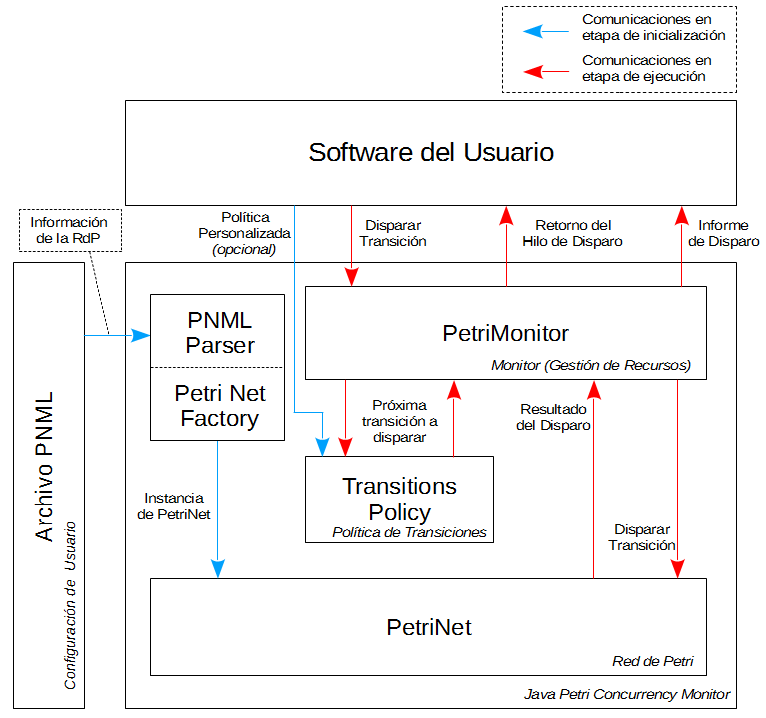
\includegraphics[width=0.8\textwidth]{JPCM_Arquitectura}
  \caption{Arquitectura de JPCM}
  \label{fig:JPCM_Arquitectura}
\end{figure}

\subsection{Gestión de los Recursos con RdP}
\label{JPCM_gestion_rec_rdp}
En la sección \ref{monitores} se analiza cómo se gestionan los recursos de un
monitor con variables de condición en un monitor de sincronización explícita.
En dicha sección se explicó cómo un hilo que desea tomar o devolver un recurso
debe señalizar a una variable de condición, y bloquearse en caso de no tener el
recurso disponible.

Por otro lado, en la sección \ref{POPN} se explica cómo una RdP representa
procesos. De esta manera, para ejecutar un proceso \textit{A}, un hilo debe
señalizar el comienzo y fin de la ejecución en la RdP disparando un subconjunto
de transiciones de inicio y otro subconjunto de transiciones de finalización.
 
De esta forma se establece una relación entre las operaciones de una variable de
condición y los disparos de una transición. Se logra obtener el mismo
comportamiento sobre los hilos que las acceden con la ayuda de colas auxiliares. 

El intento de disparo sobre una transición no sensibilizada es equivalente a una
llamada a \textit{signal()} sobre una variable de condición (ver sección
\ref{variables_condicion}).
De la misma manera, el disparo de una transición que resulta en la
sensibilización de otra, es equivalente a una llamada a \textit{signal()} sobre
una variable de condición.

Por inducción podemos decir que una variable de condición verdadera equivale a
disparar una transición y una variable de condición falsa equivale a no poder
disparar una transición.

A aprtir de esta semejanza queda en evidencia que las operaciones a realizar
dentro de un monitor que ejecuta una RdP consisten consisten del disparo de
transiciones para evolucionar el estado de los recursos y operaciones del
sistema modelado.

\subsection{Estructura Interna de JPCM}
Basándose en el diagrama de la figura \ref{fig:JPCM_Arquitectura}, se puede
dividir a JPCM en dos secciones:
\begin{itemize}
    \item Modelo: Tiene como eje central a la clase \textit{PetriNet}.
    Dentro de esta sección está el modelo a ejecutar. Contiene las matrices de
    la RdP (parte estática del modelo) y al vector de estado (parte dinámica).
    Define y expone el método de cambio de estado (disparo de una transición).
    \item Conducción: Tiene como eje central a la clase \textit{PetriMonitor}.
    Se encarga de conducir a los hilos que ejecutan el modelo.
    Incluye clases auxiliares para implementar las políticas del monitor (de
    transiciones y de colas).
\end{itemize}

\subsubsection{Sección Modelo}
En el diagrama de la figura \ref{fig:JPCM_PetriNet_Structure} se observan las
clases que componen a esta sección, sus relaciones y colaboraciones:

\begin{figure}[H]
  \centering
  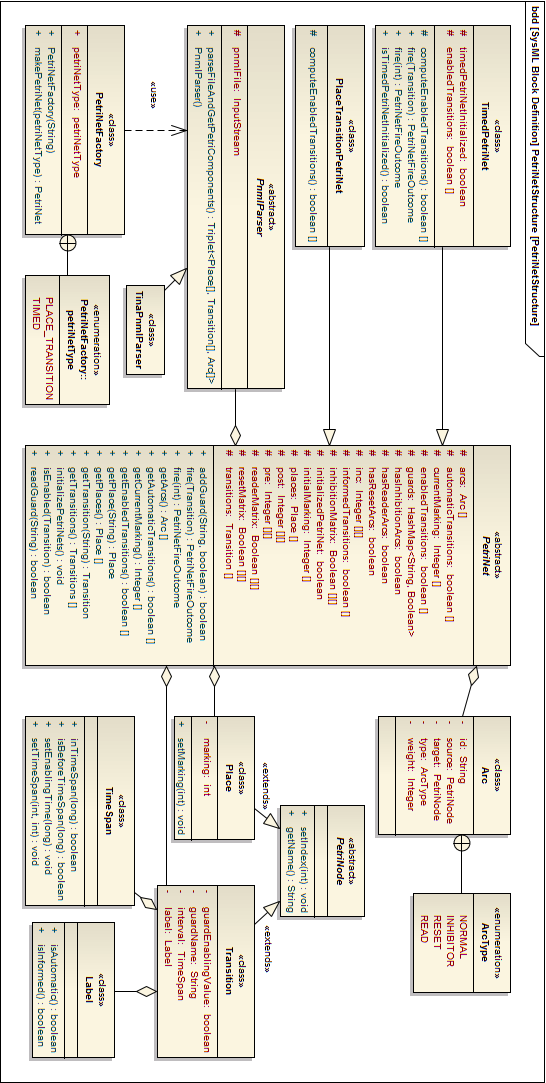
\includegraphics[height=\textheight]{JPCM_PetriNet_Structure_Simple}
  \caption{Diagrama de clases de la sección \textit{Modelo}}
  \label{fig:JPCM_PetriNet_Structure}
\end{figure}

Se observan las clases que modelan a los componentes de una RdP estructural
(ver sección \ref{def_formal_petri}) (\textit{Arc}, \textit{Transition},
\textit{Place}), la especializaciones concretas de \textit{PetriNet}
(\textit{PlaceTransitionPetriNet} para RdP plaza-transición y
\textit{TimedPetriNet} para RdP temporales), las clases \textit{PetriNetFactory}
y \textit{PnmlParser} analizadas en la sección \ref{JPCM_arq_alto_nivel} y la
especialización de \textit{PnmlParser} que comprende el dialecto PNML de TINA,
\textit{TinaPnmlParser}. Además se observan las relaciones entre estas clases
que colaboran entre sí.

\subsubsection{Sección Conducción}
En el diagrama de la figura \ref{fig:JPCM_PetriMonitor_Structure} se observan
las clases que componen a esta sección, sus relaciones y colaboraciones:

\begin{figure}[H]
  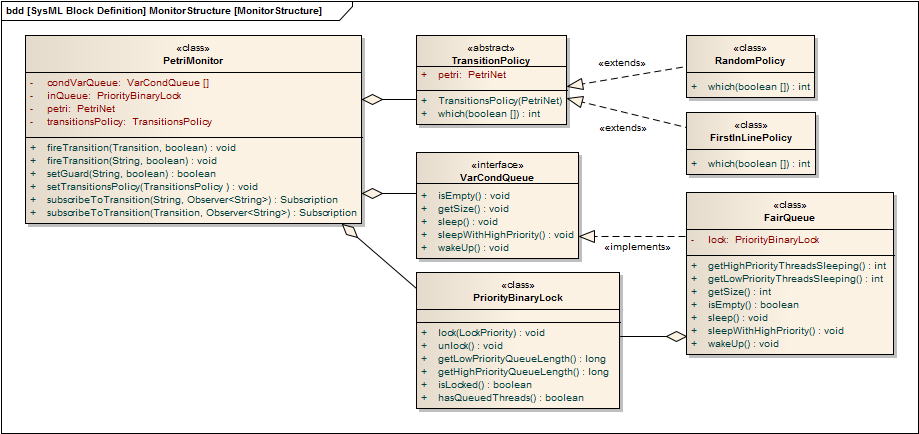
\includegraphics[width=\textwidth]{JPCM_PetriMonitor_Structure_Simple}
  \caption{Diagrama de clases de la sección \textit{Conducción}}
  \label{fig:JPCM_PetriMonitor_Structure}
\end{figure}

Junto a la clase \textit{PetriMonitor} se puede ver por un lado la subsección
que aplica la política de transiciones. Esta subsección contiene la clase
abstracta \textit{TransitionsPolicy}, cuya responsabilidad es elegir cuál
transición disparar dado un conjunto de transiciones sensibilizadas.
Se proveen dos especializaciones: 
\begin{itemize}
  \item \textit{RandomPolicy}: Política aleatoria. Basa su decisión en un
  generador de números aleatorios.
  \item \textit{FirstInLinePolicy}: Política de primer transición en la lista.
  Elige siempre a la primer transición sensibilizada que encuentre en la lista.
\end{itemize}

Por otro lado, la clase \textit{PriorityBinaryLock} implementa la política de
colas por prioridad (ver sección \ref{JPCM_solucion_inv_prioridad}) y es
utilizada tanto para la cola de entrada como para las colas de condición.

Las colas de condición asociadas a las transiciones (ver sección
\ref{JPCM_gestion_rec_rdp}) están descriptas en la interfaz
\textit{VarCondQueue} e implementadas en la clase \textit{FairQueue}.


\subsection{Interfaces de Programación}

JPCM ofrece una interfaz de entrada al monitor y dos de salida en tiempo de
ejecución, y dos interfaces de carga de datos de configuración en tiempo de
inicialización.

En tiempo de ejecución, la interfaz de entrada es el método público 
\mint{java}|PetriMonitor.fireTransition()|. Este método permite disparar una
transición de la RdP dentro del monitor de concurrencia, ya sea utilizando el
objeto \textit{Transition} (transición) de la RdP, o el nombre de la misma.

Las interfaces salida son dos:
\begin{itemize}
  \item \underline{Retorno del disparo de una transición:} la finalización de
  ejecución del método \mint{java}|PetriMonitor.fireTransition()| asegura que el
  hilo que hizo la llamada, efectivamente disparó de la transición deseada
  (excepto en disparos no-perennes donde no se desea esta garantía, ver sección
  \ref{disparos_perennes})
  \item \underline{Informes de disparo:} ante el disparo de una
  transición informada, se emite un evento con información sobre la transición
  disparada. Todos los observadores suscritos a estos eventos lo recibirán.
\end{itemize}

En tiempo de inicialización se proveen dos interfaces al usuario:
\begin{itemize} 
  \item \underline{Carga de una RdP:} Se hace mediante un archivo descriptor
  en formato PNML. El bloque \textit{PnmlParser + PetriNetFactory} lo utiliza
  para generar una RdP ejecutable.
  \item \underline{Carga de una política personalizada:} Es opcional. Permite
  al usuario definir una política de transiciones que se ajuste al problema a
  resolver por su software.
\end{itemize}

Estas interfaces proveen al usuario de los mecanismos necesarios para
inicializar el monitor, y para luego utilizarlo.

\subsection{Inicialización de JPCM}
Los pasos para inicializar JPCM son:
\begin{itemize}
  \item Instanciar la clase \textit{PnmlParser} con la ruta al archivo de
  descripción de la RdP a utilizar
  \item Instanciar la clase \textit{PetriNetFactory} con el objeto
  \textit{PnmlParser}
  \item Utilizar el objeto \textit{PetriNetFactory} para generar una instancia
  de \textit{PetriNet}
  \item Instanciar una política (clases \textit{FirstInLinePolicy} o
  \textit{RandomPolicy} o la desarrollada por el usuario)
  \item Instanciar la clase \textit{PetriMonitor} con el objeto
  \textit{PetriNet} y el objeto de la política
  \item Crear los hilos que van a ejecutar las acciones del sistema
  \item Inicializar la RdP llamando a \mint{java}|PetriNet.initializePetriNet()|
  sobre la instancia de \textit{PetriNet}
  \item Lanzar los hilos creados anteriormente
  \item Evitar que el hilo principal termine antes que los hilos trabajadores
\end{itemize}
 
Luego de realizar todas estas tareas, el sistema se ejecuta guiado por la RdP.

\subsubsection{Generación de una RdP Ejecutable a Partir de un Archivo PNML}
Como se dijo anteriormente, JPCM requiere de un archivo PNML con la descripción
de la RdP a utilizar. Los pasos a seguir para obtener una RdP ejecutable a
partir del archivo PNML son los siguientes:
\begin{itemize}
  \item Una instancia de PnmlParser analiza el archivo para obtener los
  componentes de RdP contenidos en él (Plazas, Arcos y Transiciones)
  \item Con la información obtenida genera objetos de tipo \textit{Place},
  \textit{Transition} o \textit{Arc} dependiendo del caso
  \item Ordena los objetos generados en tres arrays, uno por cada tipo de
  componente y los empaqueta en una tupla
  \item Cuando se llama a \mint{java}|PetriNetFactory.makePetriNet()| sobre la
  instancia de \textit{PetriNetFactory}, ésta obtiene la tupla de arrays de
  componentes generada por \textit{PnmlParser}
  \item Con los objetos componentes de la RdP, \textit{PetriNetFactory} calcula
  y almacena las matrices de precedencia, pos-incidencia, incidencia, inhibición,
  reset y lectura, y el vector del marcado inicial
  \item Con los objetos componentes, las matrices de la RdP y el tipo de RdP a
  generar, crea una instancia de la subclase de \textit{PetriNet}
  correspondiente (\textit{TimedPetriNet} para RdP temporales y
  \textit{PlaceTransitionPetriNet} para RdP ordinarias)
\end{itemize}

El objeto resultante es una RdP ejecutable que se utiliza en conjunto con el
monitor.

\subsection{Disparo de una Transición en JPCM}
El disparo de una transición en el monitor mediante la ejecución del método
\mint{java}|PetriMonitor.fireTransition(t)| desencadena las siguientes acciones
sobre el hilo que realiza la llamada:

\begin{itemize}
  \item \underline{Verifica que la transición t no sea automática:} En cuyo caso
  falla con un error explicando la situación
  \item \underline{Verifica que la red esté inicializada:} En caso contrario
  falla con un error explicando la situación
  \item \underline{Toma el lock sobre la entrada del monitor:} Si no lo puede
  tomar se bloquea en la cola de entrada hasta poder tomarlo
  \item  \underline{Dispara la transición en la RdP:} Devuelve un código de
  estado indicando el resultado (ver sección \ref{codigos_de_estado_disparo})
  \item \underline{Maneja el resultado del disparo:} se analiza si se debe
  liberar el lock de entrada, disparar una transición automática, liberar un
  hilo bloqueado o bloquearse por una condición
  \item \underline{Libera el lock de entrada:} Sólo si es necesario. Algunas
  situaciones requieren que no se permita la entrada de un nuevo hilo, como la
  liberación de un hilo bloqueado en una cola de condición
\end{itemize}
 
La figura \ref{fig:JPCM_Fire_General} es un diagrama de secuencias donde se
muestra el flujo de un hilo que realiza un disparo de una transición:

\begin{figure}[H]
  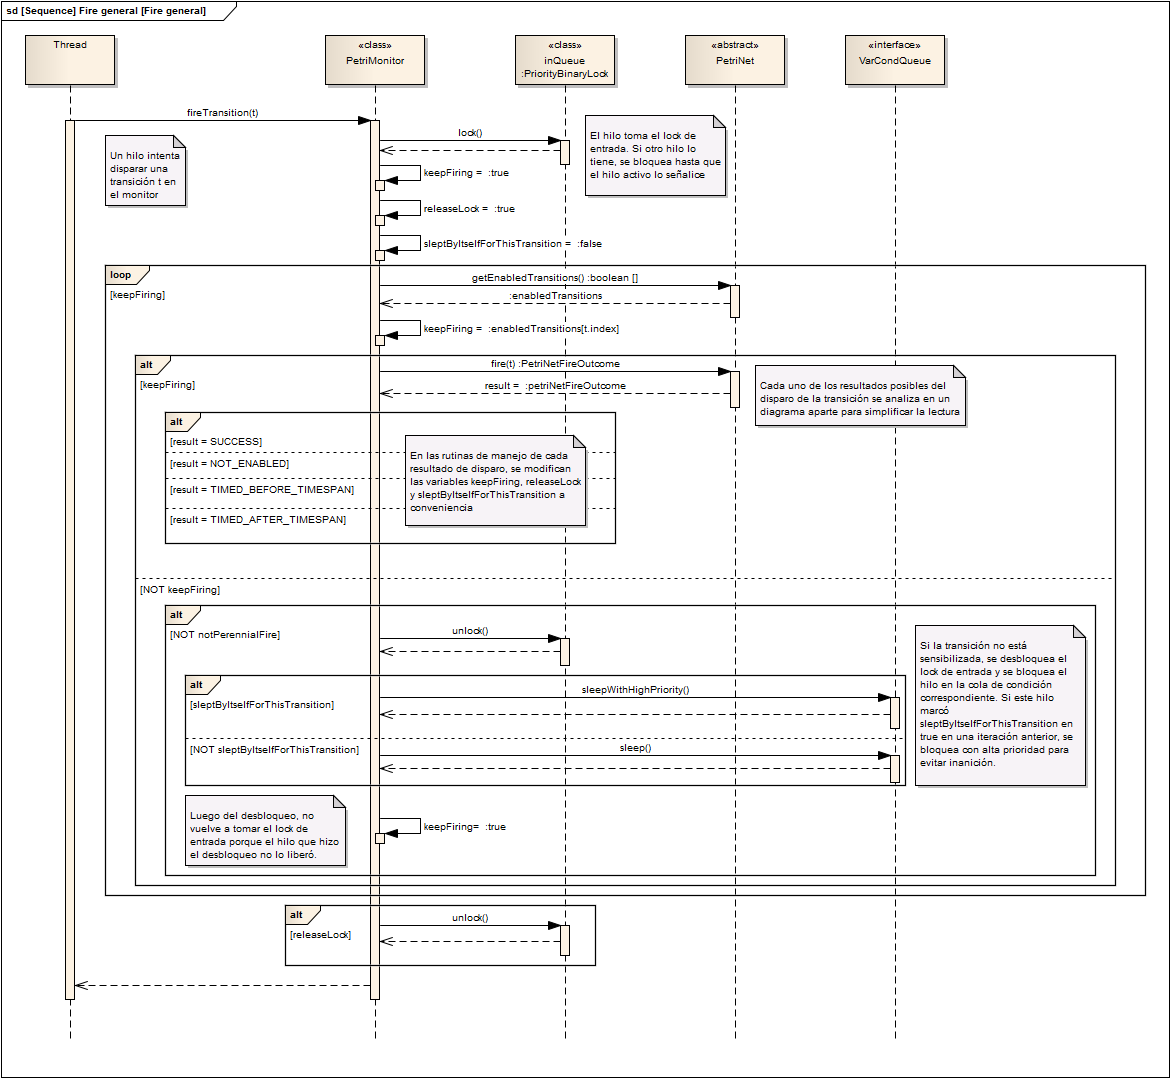
\includegraphics[width=\textwidth]{JPCM_Fire_General}
  \caption{Disparo de una transición}
  \label{fig:JPCM_Fire_General}
\end{figure}

\subsection*{Manejo del código de estado del disparo}
\label{codigos_de_estado_disparo}

Cuando se realiza el disparo efectivo de la transición en la Red de Petri, ésta
devuelve un código de estado, que es el resultado del disparo. Estos pueden
ser:
\begin{itemize}
  \item \textit{SUCCESS:} el disparo fue exitoso
  \item \textit{NOT\_ENABLED:} la transición no está sensbilizada
  \item \textit{TIMED\_BEFORE\_TIMESTAMP:} Sólo para transiciones
  temporales. El instante de disparo es anterior al \textit{instante menor de
  disparo} $(\alpha)$ de la transición (ver sección \ref{semantica_tiempo_debil})
  \item \textit{TIMED\_AFTER\_TIMESTAMP:} Sólo para transiciones
  temporales. El instante de disparo es posterior al \textit{instante mayor de
  disparo} $(\beta)$ de la transición (ver sección \ref{semantica_tiempo_debil})
\end{itemize}

\subsubsection*{Caso del disparo exitoso}
Ante un disparo exitoso, la llamada a \mint{java}|PetriNet.fire(Transition t)|
devuelve un código \textit{SUCCESS}. Una vez que esto ocurre, el hilo que
realizó el disparo debe:
\begin{itemize}
  \item Emitir un evento para todos los suscriptores (en el caso que la
  transición sea informada).
  \item Determinar si existen nuevas transiciones sensibilizadas producto del
  último disparo
      \begin{itemize}
        \item Si no existen, libera el lock de entrada y abandona el monitor
        \item Si existen:
            \begin{itemize}
                \item Selecciona a la próxima transición $t_{n}$ a ser
                disparada, de acuerdo con la política de transiciones.
                \item Si $t_{n}$ es de tipo \textit{automática} el disparo lo
                hace el mismo hilo, por lo que itera para realizar un nuevo
                disparo sobre dicha transición.
                \item Si $t_{n}$ es de tipo \textit{disparada} se debe
                señalizar al hilo que esté esperando en su cola de condición y
                abandonar el monitor inmediatamente sin liberar el lock de entrada.
            \end{itemize}
      \end{itemize}
\end{itemize}

En el diagrama de secuencias de la figura \ref{fig:JPCM_Fire_SUCCESS} se observa
en detalle el flujo de un disparo exitoso de una transición:

\begin{figure}[H]
  \centering
  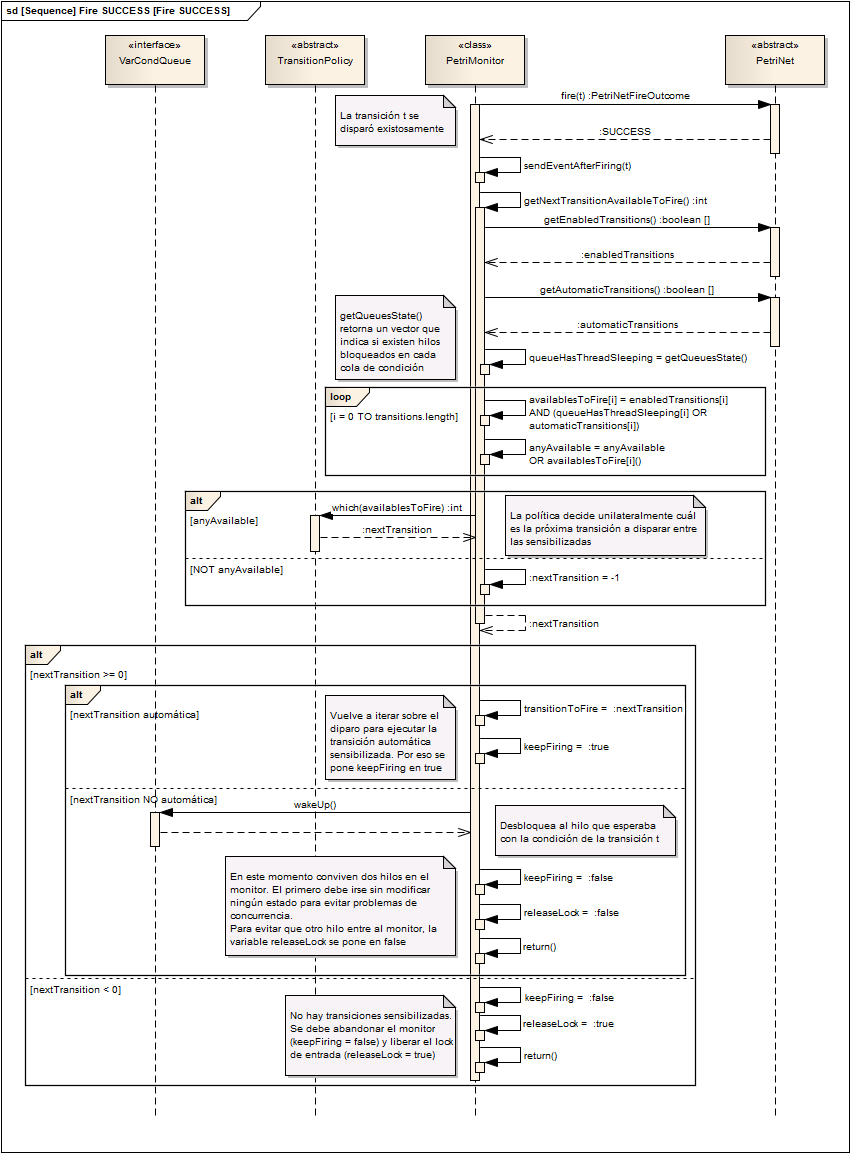
\includegraphics[width=0.85\textwidth]{JPCM_Fire_SUCCESS}
  \caption{Manejo del disparo exitoso de una transición}
  \label{fig:JPCM_Fire_SUCCESS}
\end{figure}

\subsubsection*{Caso del disparo no exitoso}

Cuando la transición no está sensibilizada, su disparo devuelve
\textit{NOT\_ENABLED}. Ante este caso, un hilo que realizó un disparo perenne
debe esperar en la cola de condición asociada a la transición. A su vez, si en
una iteración anterior realizó una espera temporal por la transición, debe
bloquearse con alta prioridad.
 
En el diagrama de secuencias de la figura \ref{fig:JPCM_Fire_NOT_ENABLED} se muestra
detallado el caso del disparo no exitoso.

\begin{figure}[H]
  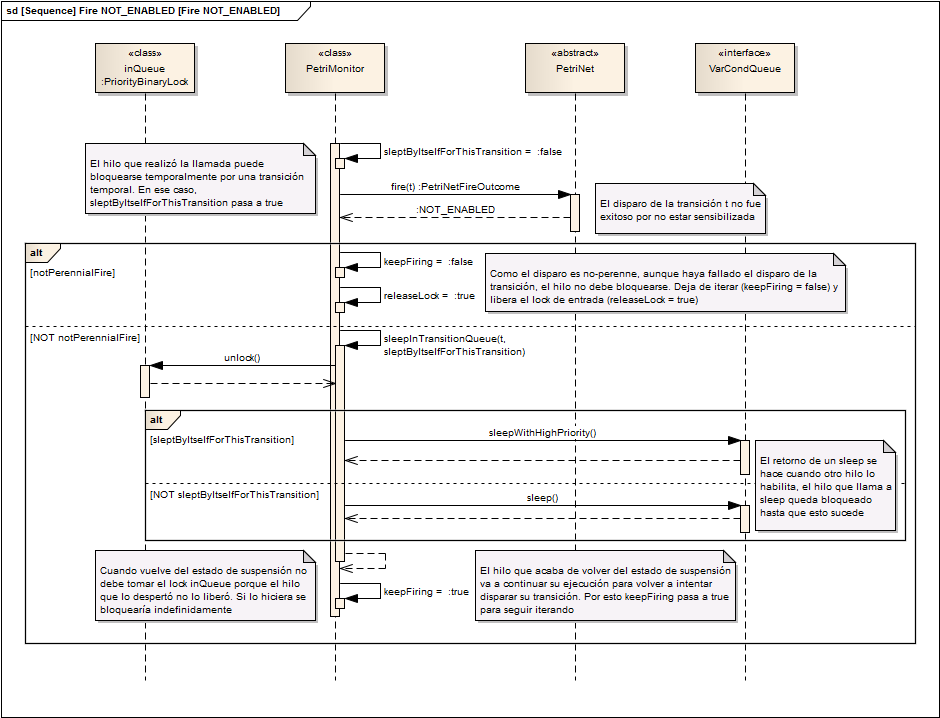
\includegraphics[width=\textwidth]{JPCM_Fire_NOT_ENABLED}
  \caption{Manejo del disparo no exitoso de una transición}
  \label{fig:JPCM_Fire_NOT_ENABLED}
\end{figure}

\subsubsection*{Caso del disparo temporal antes del intervalo}
Si un hilo intenta disparar una transición temporal antes del instante menor de
disparo, la llamada a \mint{java}|PetriNet.fire(t)| devuelve un código de estado
\textit{TIMED\_BEFORE\_TIMESPAN}.
En este caso, el procedimiento a seguir es el siguiente:
\begin{itemize}
  \item Si no hay hilo bloqueado por t:
      \begin{itemize}
        \item Liberar el lock de entrada
        \item Esperar temporalmente hasta el \textit{instante menor de disparo}
        \item Tomar el lock de entrada con alta prioridad (ver
        sección~\ref{sec:inversion_prioridad})
        \item Señalizar que ya se suspendió temporalmente para evitar futuras
        inversiones de prioridad
        \item Iterar sobre el disparo para reintentarlo
      \end{itemize}
  \item Si existe un hilo bloqueado por t:
      \begin{itemize}
        \item Si el disparo es no-perenne
                \begin{itemize}
                  \item Liberar el lock de entrada
                  \item Abandonar el monitor
                \end{itemize}
        \item Si el disparo es perenne
                \begin{itemize}
                  \item Liberar el lock de entrada
                  \item Bloquearse en la cola de condición de t. Si ya se suspendió
                  temporalmente por t antes, lo hace con alta prioridad (ver
                  sección~\ref{sec:inversion_prioridad})
                  \item Cuando se desbloquea itera para reintentar el disparo
                \end{itemize}
      \end{itemize}
\end{itemize}
En el diagrama de secuencias de la figura
\ref{fig:JPCM_Fire_TIMED_BEFORE_TIMESPAN} se detalla el flujo de este caso de
resultado de disparo.

\begin{figure}[H]
  \centering
  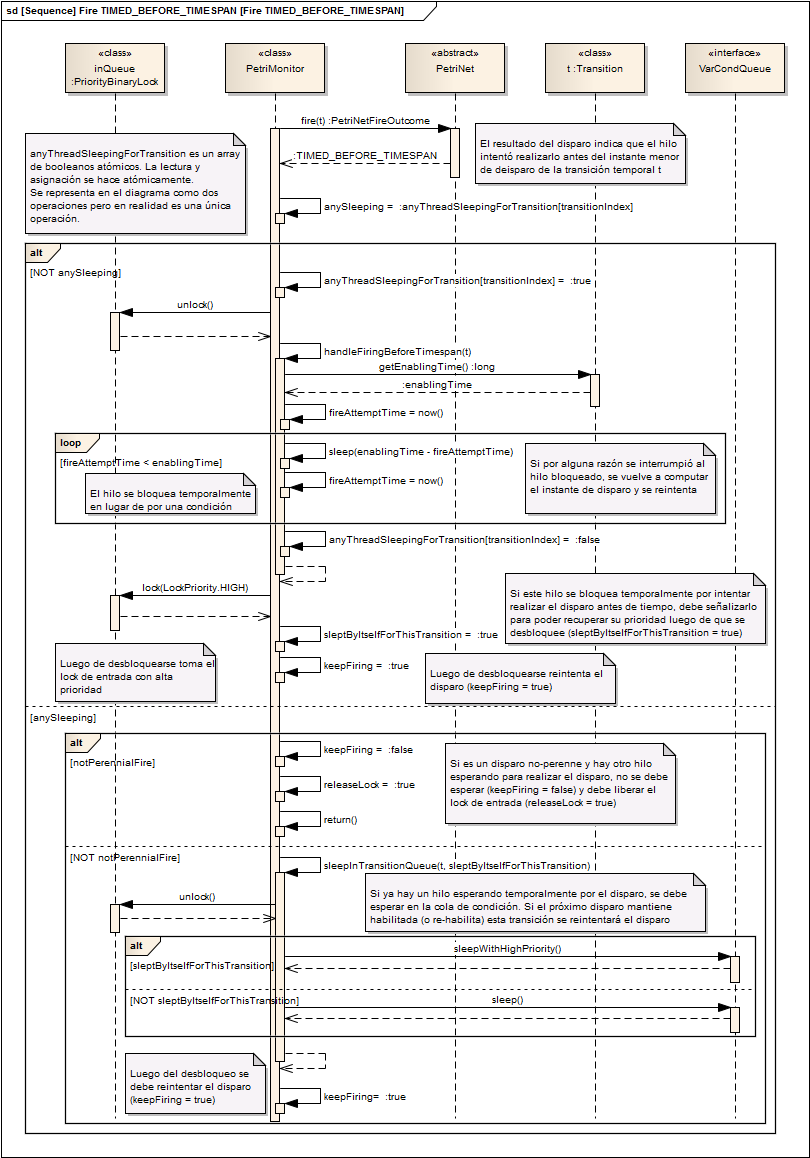
\includegraphics[width=0.85\textwidth]{JPCM_Fire_TIMED_BEFORE_TIMESPAN}
  \caption{Manejo del disparo de una transición temporal antes del instante
  menor de disparo}
  \label{fig:JPCM_Fire_TIMED_BEFORE_TIMESPAN}
\end{figure}

\subsubsection*{Caso del disparo temporal después del intervalo}

Ante el intento de disparo de una transición temporal en un instante posterior
al instante mayor de disparo, el resultado es \textit{TIMED\_AFTER\_TIMESPAN}.
Al no cumplirse la condición de sensibilización temporal, este intento de
disparo es equivalente al caso del disparo no exitoso. Por esto, la rutina de
manejo de ambos casos es la misma y correponde al diagrama de secuencias de la
figura \ref{fig:JPCM_Fire_NOT_ENABLED}.

\subsection{Problema de la Inversión de Prioridades}
\label{sec:inversion_prioridad}
Durante el desarrollo de JPCM se detectaron dos casos donde se produce una
inversión de prioridades entre los hilos gestionados. A continuación se
analizan estos casos.

\subsubsection{Inversión de prioridades en la cola de entrada}
\label{inversion_prioridad_cola_entrada}
Existe inversión de prioridad en la cola de entrada si ocurren los siguientes
eventos en orden:
\begin{itemize}
  \item Se sensibiliza la transición temporal $t_{0}$ con intervalo $[a,b]$ en
  el instante $t_{i}$
  \item El hilo $th_{0}$ intenta disparar $t_{0}$ en $t_{d} < (t_{i} + a)$
  \item El hilo $th_{0}$ libera la entrada y se bloquea temporalmente
  \item Entra otro hilo a realizar un disparo y bloquea la entrada
  \item Llegan al monitor $N$ hilos a intentar realizar disparos y se encolan a
  la entrada
  \item Cuando $th_{0}$ se desbloquea, intenta tomar el lock de entrada y va al
  final de la cola
\end{itemize}

En este caso, $th_{0}$ cedió su prioridad a los $N$ hilos que llegaron después
que él. Esto provoca que el intervalo de disparo termine antes de que $th_{0}$
recupere su turno dentro del monitor, provocando su inanición.

La figura \ref{fig:Inv_prior_entrada} explica esta secuencia. Está formada por
una sucesión de subfiguras, una por cada instante de interés. Los elementos que
aparecen en todas ellas son:
\begin{itemize}
    \item El monitor de concurrencia (rectángulo mayor)
    \item La cola de entrada
    \item Las colas de condición
    \item Una Red de Petri con tres plazas y cuatro transiciones, donde $t_{0}$
    es temporal con intervalo $[\alpha,\beta]$
    \item Un reloj que indica en instante de cada subfigura
    \item Un área donde se simboliza el bloqueo temporal de un hilo (rectángulo
    redondeado con líneas de punto)
    \item Uno o más hilos. El hilo rojo es el de interés
\end{itemize}

Las subfiguras grafican los siguientes eventos:
\begin{enumerate}[label=\alph*)]
    \item La transición $t_{0}$ se sensibiliza en el instante $t_{i}$. Luego, el
    hilo $th_{0}$ llama a \mint{java}|petriMonitor.fireTransition("t0")|. 
    \item Como no hay hilo activo en el monitor y la cola de entrada está vacía,
    $th_{0}$ toma el lock de entrada e intenta disparar $t_{0}$. Mientras tanto
    se encolan algunos hilos en la cola de entrada
    \item La llamada a \mint{java}|petri.fire("t0")| retornó un código
    \mint{java}|TIMED_BEFORE_TIMESPAN|, por lo que $th_{0}$ se bloquea
    temporalmente hasta el instante $t_{i}+a$.
    \item Antes de bloquearse, $th_{0}$ libera la entrada al monitor. Otro hilo
    ingresa al monitor a disparar a $t_{1}$
    \item Se alcanza el instante $t_{i}+a$ por lo que $th_{0}$ se desbloquea y
    reintenta el disparo. Como la cola de entrada no está vacía, se encola al
    final
    \item Otro hilo ingresa al monitor a disparar a $t_{2}$
    \item Se superó el instante $t_{i}+b$ (fin del intervalo de disparo de
    $t_{0}$) sin que $th_{0}$ haya podido hacer el disparo, provocando su
    inanición
\end{enumerate}

\begin{figure}[H]
    \centering
    \ContinuedFloat
    \subfigure[] {
      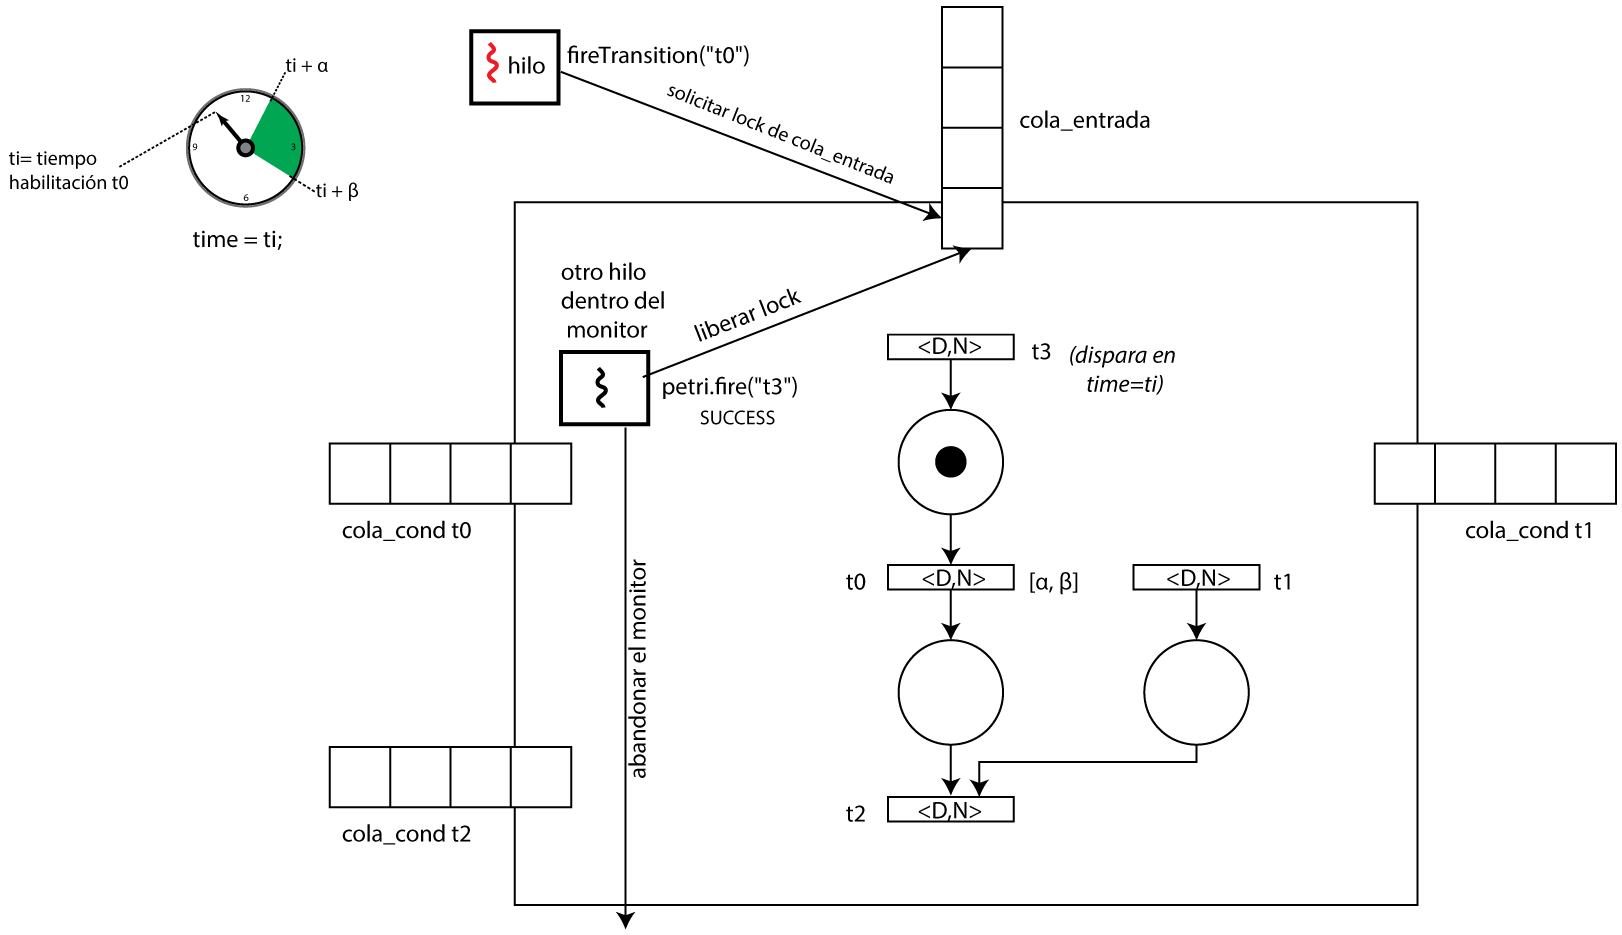
\includegraphics[width=\textwidth]{InversionPrioridad/Inversion_Prioridad_01}
    }
    \phantomcaption
    \label{fig:Inv_prior_entrada}
\end{figure}
\begin{figure}[H]
    \ContinuedFloat
    \subfigure[] {
      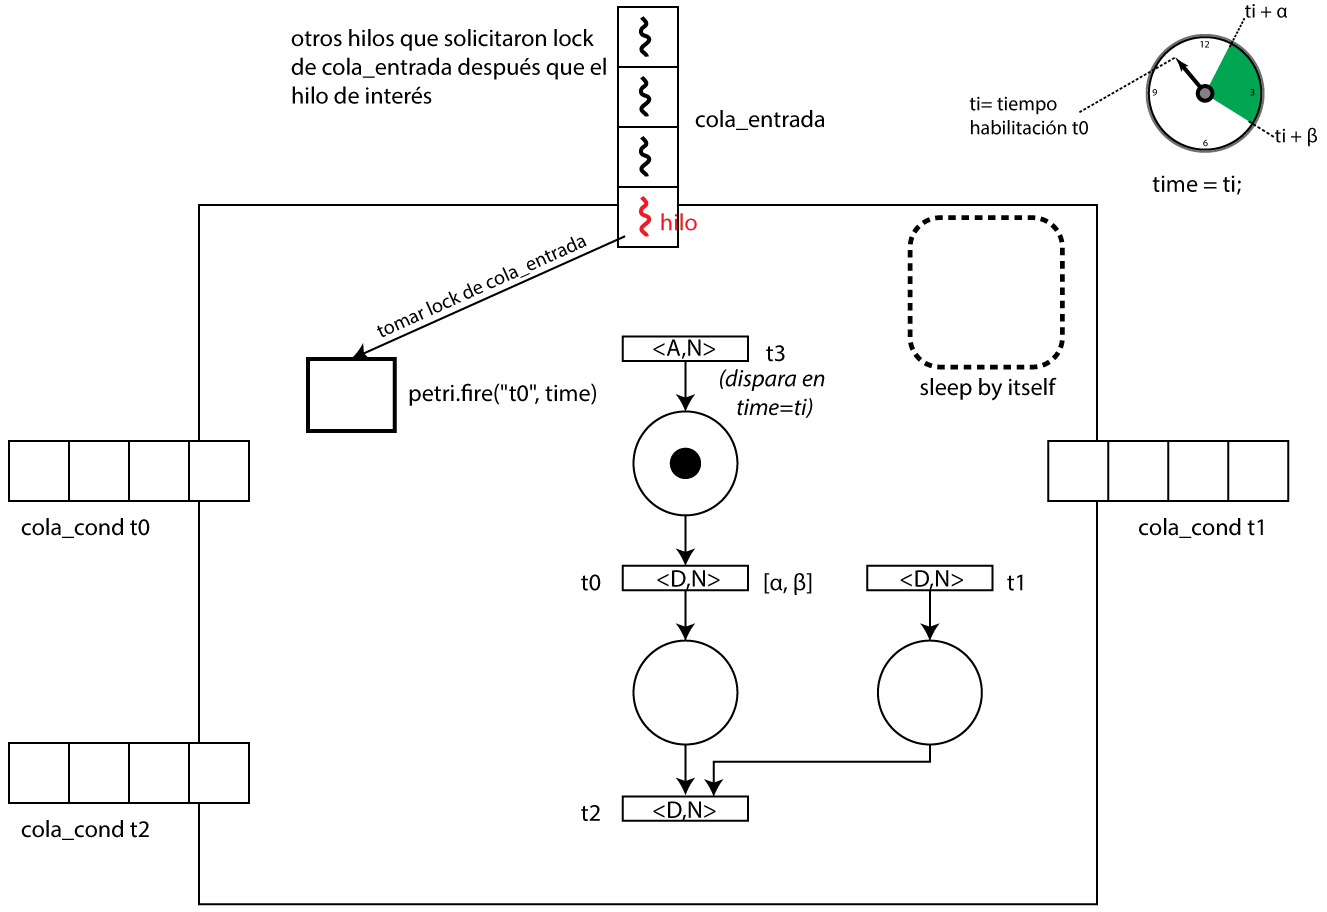
\includegraphics[width=\textwidth]{InversionPrioridad/Inversion_Prioridad_02}
    }
    \label{fig:Inv_prior_entrada}
\end{figure}
\begin{figure}[H]
    \ContinuedFloat
    \subfigure[] {
      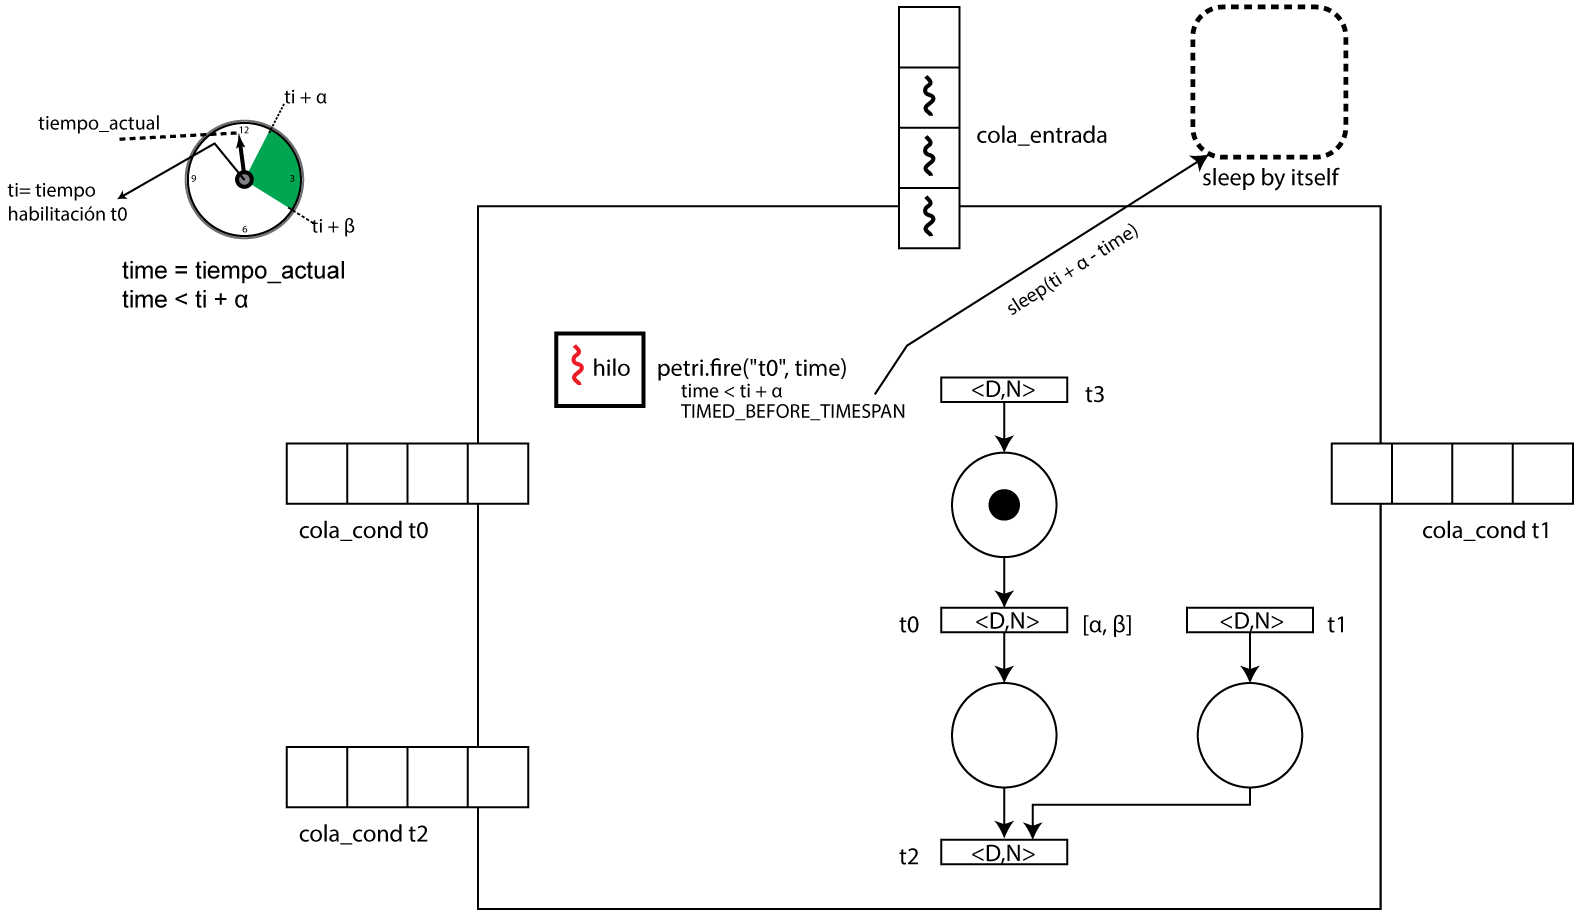
\includegraphics[width=\textwidth]{InversionPrioridad/Inversion_Prioridad_03}
    }
\end{figure}
\begin{figure}[H]
    \ContinuedFloat
    \subfigure[] {
      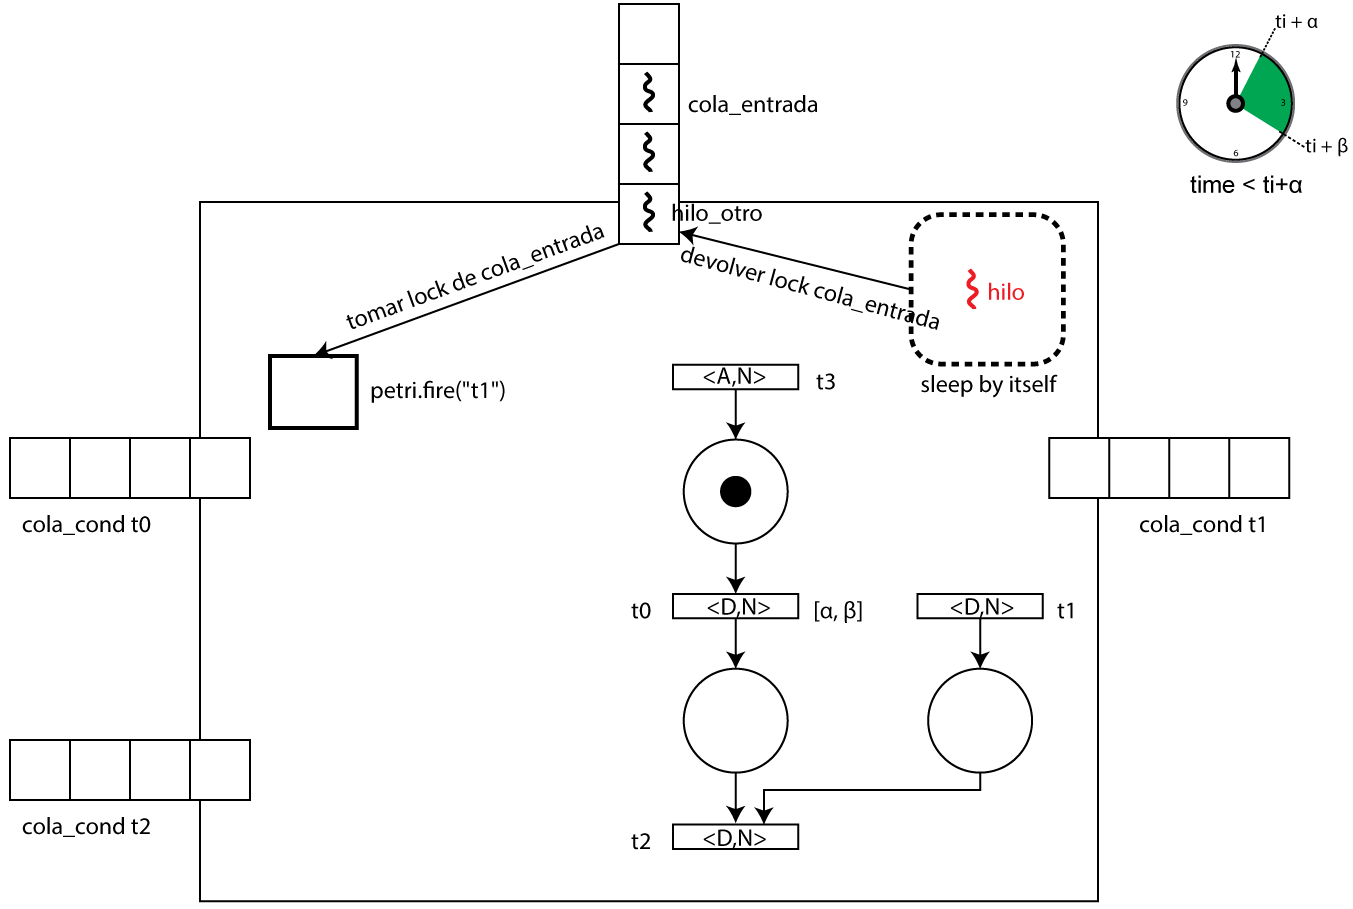
\includegraphics[width=\textwidth]{InversionPrioridad/Inversion_Prioridad_04}
    }
    \label{fig:Inv_prior_entrada}
\end{figure}
\begin{figure}[H]
    \ContinuedFloat
    \subfigure[] {
      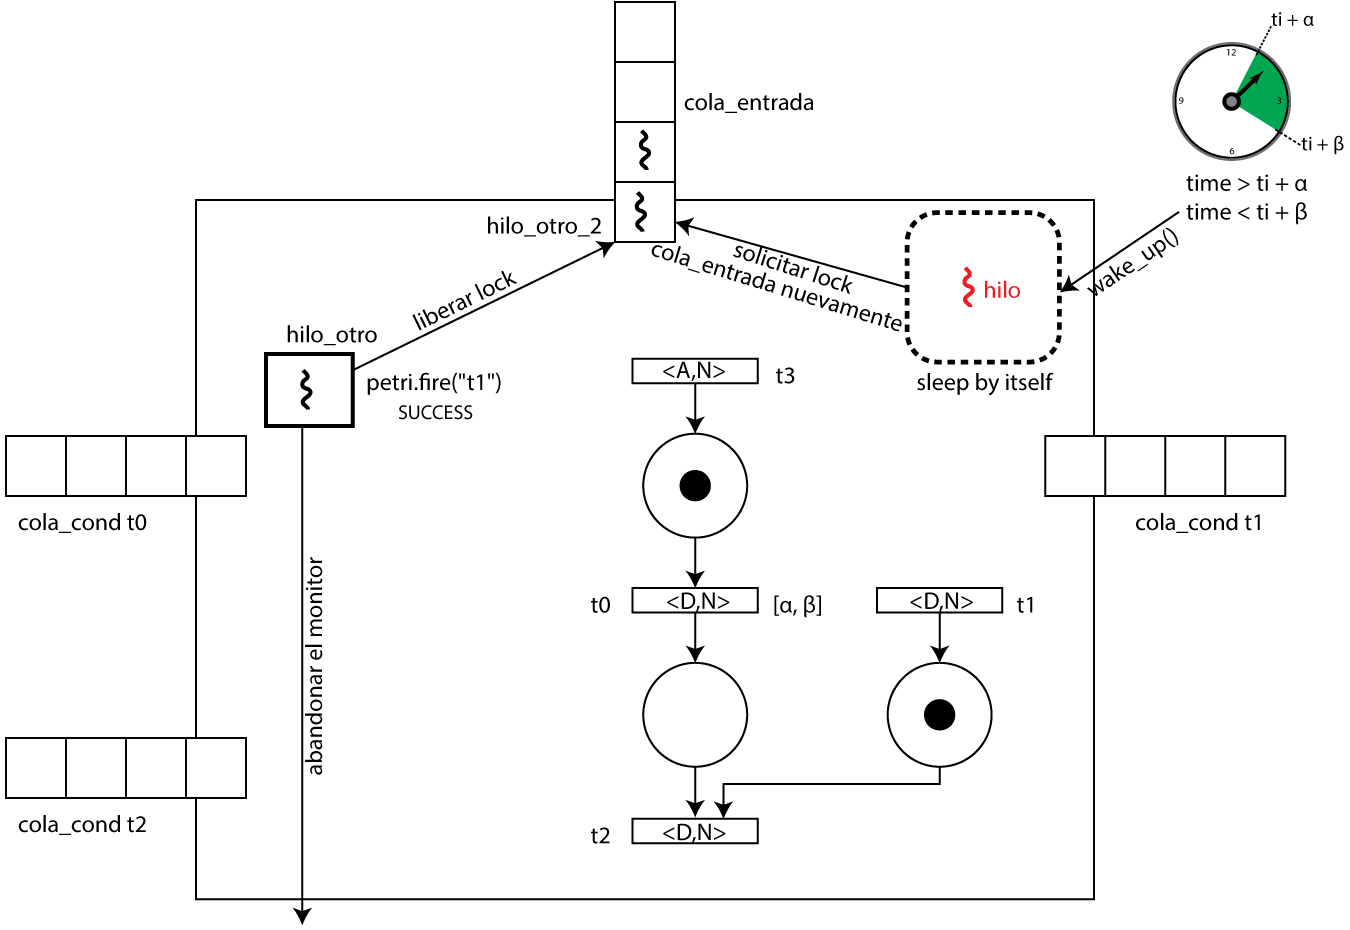
\includegraphics[width=\textwidth]{InversionPrioridad/Inversion_Prioridad_05}
    }
\end{figure}
\begin{figure}[H]
    \ContinuedFloat
    \subfigure[] {
      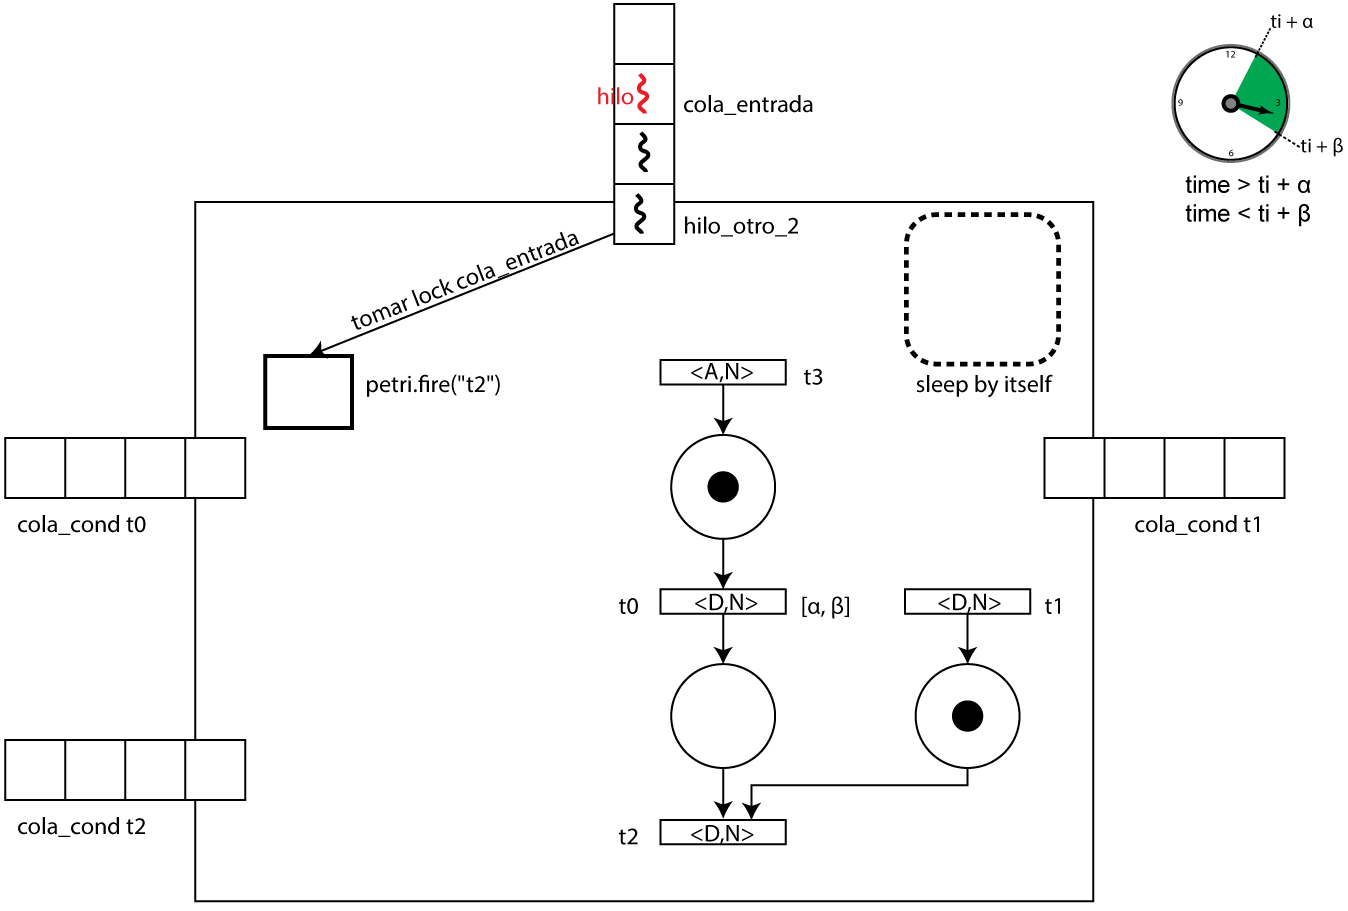
\includegraphics[width=\textwidth]{InversionPrioridad/Inversion_Prioridad_06}
    }
    \label{fig:Inv_prior_entrada}
\end{figure}
\begin{figure}[H]
    \ContinuedFloat
    \subfigure[] {
      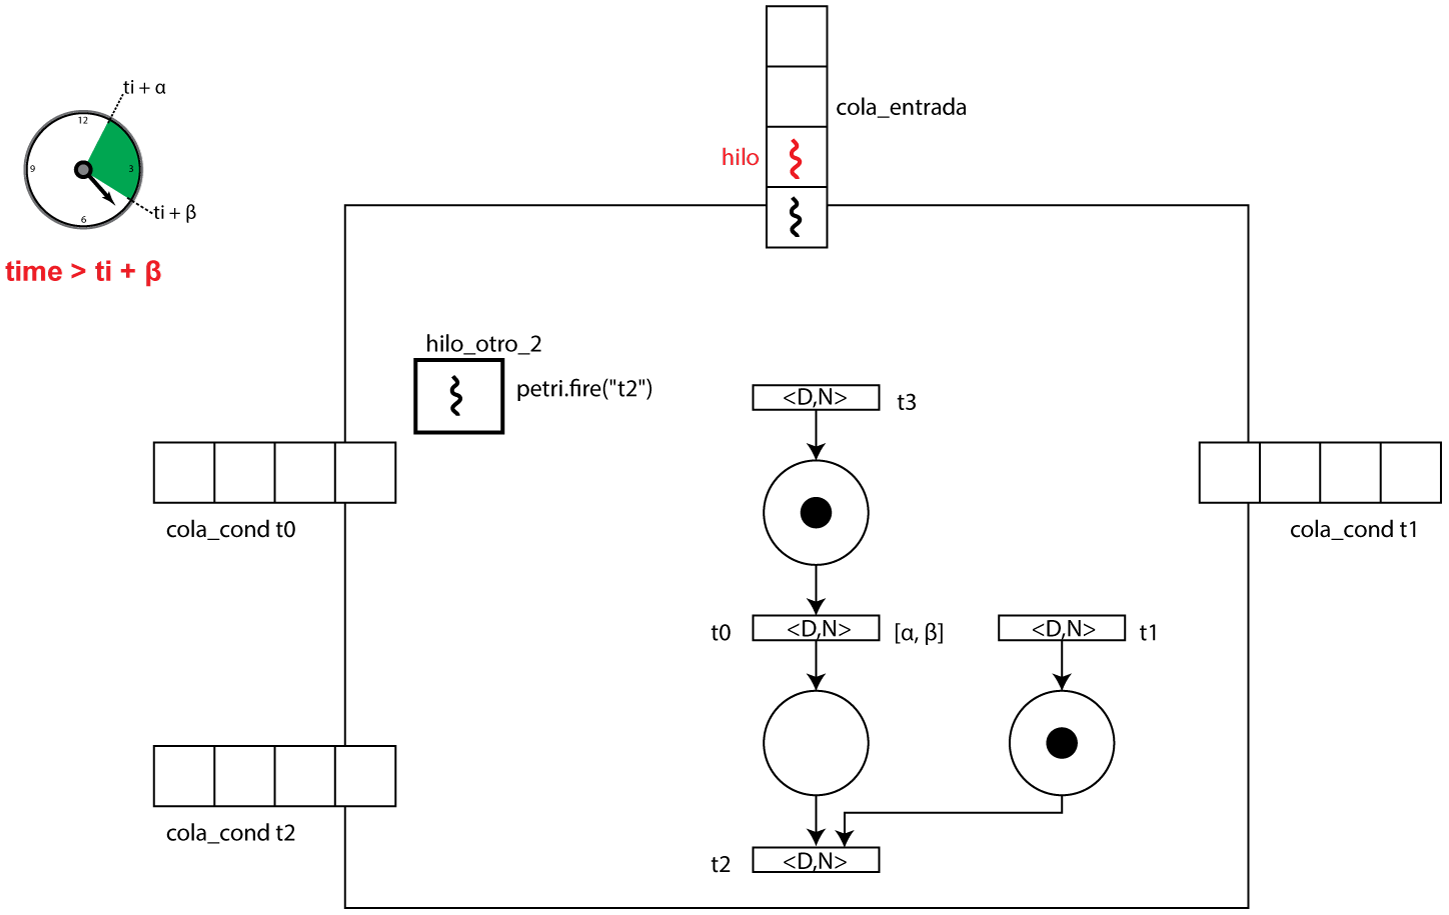
\includegraphics[width=\textwidth]{InversionPrioridad/Inversion_Prioridad_07}
    }
    \caption{Inversión de prioridades en la cola de entrada del monitor}
    \label{fig:Inv_prior_entrada}
\end{figure}

\subsubsection{Inversión de prioridades en una cola de condición}

Existe inversión de prioridad en la cola de condición de una transición si
ocurren los siguientes eventos en orden:
\begin{itemize}
  \item Se sensibiliza la transición temporal $t_{0}$ con intervalo $[a,b]$ en
  el instante $t_{i}$
  \item El hilo $th_{0}$ intenta disparar $t_{0}$ en $td < (t_{i} + a)$
  \item El hilo $th_{0}$ libera la entrada y se bloquea temporalmente
  \item Llegan $N$ hilos que intentan disparar a $t_{0}$ y se encolan en su cola
  de condición
  \item El hilo $th_{1}$ toma el lock de entrada y dispara la transición
  $t_{1}$, que deshabilita a $t_{0}$
  \item Cuando $th_{0}$ se desbloquea, toma el lock de entrada e intenta
  disparar $t_{0}$. Como la transición no está sensibilizada, $th_{0}$ se
  bloquea en la cola de condición de $t_{0}$
\end{itemize}
 
En este caso, $th_{0}$ se encola al final de la cola de condición, cediéndole
incorrectamente su prioridad a los $N$ hilos que llegaron después que él al
monitor a disparar a $t_{0}$.

\subsection{Solución a los problemas de inversión de prioridad}
\label{JPCM_solucion_inv_prioridad}

Del análisis de los casos de inversión de prioridades expuestos en la sección
anterior, se llega a la conclusión de que ambos problemas se solucionan mediante
una modificación de la política de prioridad de desbloqueo de hilos en las colas
de entrada y de condición. De esta manera, un hilo que espera por la
sensibilización temporal de una transición temporizada tendrá máxima prioridad
al momento de reintentar un disparo fallido.

Para implementar colas de prioridad, \mint{java}|PetriMonitor| utiliza una
instancia de la clase \mint{java}|PriorityBinaryLock| para la cola de entrada,
y \mint{java}|FairQueue| utiliza una para las colas de condición. (ver figura
\ref{fig:JPCM_PetriMonitor_Structure}).
Esta clase define un lock que implementa dos métodos básicos para su uso:
\begin{itemize}
  \item \mint{java}|lock(LockPriority priority)|: Su parámetro es opcional y por
  defecto es de baja prioridad. Permite a un hilo tomar el lock. En caso de ya
  estar tomado, el hilo se bloquea en la cola asociada.
  \item \mint{java}|unlock()|: Libera el lock. Si existe al menos un hilo en la
  cola despierta al primero.
\end{itemize}

Internamente, \mint{java}|PriorityBinaryLock| utiliza una cola de prioridades
para gestionar los hilos bloqueados que almacena. De esta forma, siendo $A$ y $B$
dos hilos bloqueados en la cola de prioridades, $A$ estará más próximo a ser
desbloqueado si:
\begin{itemize}
  \item $A$ tiene mayor prioridad que $B$
  \item $A$ y $B$ tienen la misma prioridad pero el instante de bloqueo de $A$
  es menor al de $B$
\end{itemize}

De esta manera, dentro de un mismo rango de prioridades se respeta el esquema
FIFO utilizado comúnmente en una cola.

El ordenamiento de la cola es equivalente a que existan dos colas FIFO, una con
prioridad alta y otra baja. Así, cada vez que se libere el lock, se prefiere
desbloquear a un hilo en la cola de alta prioridad.

En la figura \ref{fig:Inv_prior_entrada} se observa la secuencia de pasos que
lleva a la solución del caso de inversión de prioridades de la sección
\ref{inversion_prioridad_cola_entrada}.

Las subfiguras grafican los siguientes eventos:
\begin{enumerate}[label=\alph*)]
    \item La transición $t_{0}$ se sensibiliza en el instante $t_{i}$. El hilo
    $th_{0}$ llama a \mint{java}|petriMonitor.fireTransition("t0")|
    \item Como no hay hilo activo en el monitor y la cola de entrada está vacía,
    $th_{0}$ toma el lock de entrada e intenta disparar $t_{0}$. Mientras tanto
    se encolan algunos hilos en la cola de entrada
    \item La llamada a \mint{java}|petri.fire("t0")| retornó un código
    \mint{java}|TIMED_BEFORE_TIMESPAN|, por lo que $th_{0}$ se bloquea
    temporalmente hasta el instante $t_{i}+a$
    \item Antes de bloquearse, $th_{0}$ libera la entrada al monitor. Otro hilo
    ingresa al monitor a disparar a $t_{1}$
    \item Se alcanza el instante $t_{i}+a$ por lo que $th_{0}$ se desbloquea y
    reintenta el disparo. Como existe un hilo activo se bloquea con alta
    prioridad.
    \item El hilo activo abandona el monitor y libera la entrada. Se habilita a
    $th_{0}$ por estar en la cola de alta prioridad.
    \item $th_{0}$ ingresa al monitor dentro del intervalo de sensibilización de
    $t_{0}$ para reintentar el disparo
    \item $th_0$ logró disparar a $t_{0}$ dentro del intervalo de
    sensibilización y abandona el monitor, liberando la entrada para un nuevo
    hilo
\end{enumerate}

\begin{figure}[H]
    \centering
    \ResetCounter
    \ContinuedFloat
    \subfigure[] {
      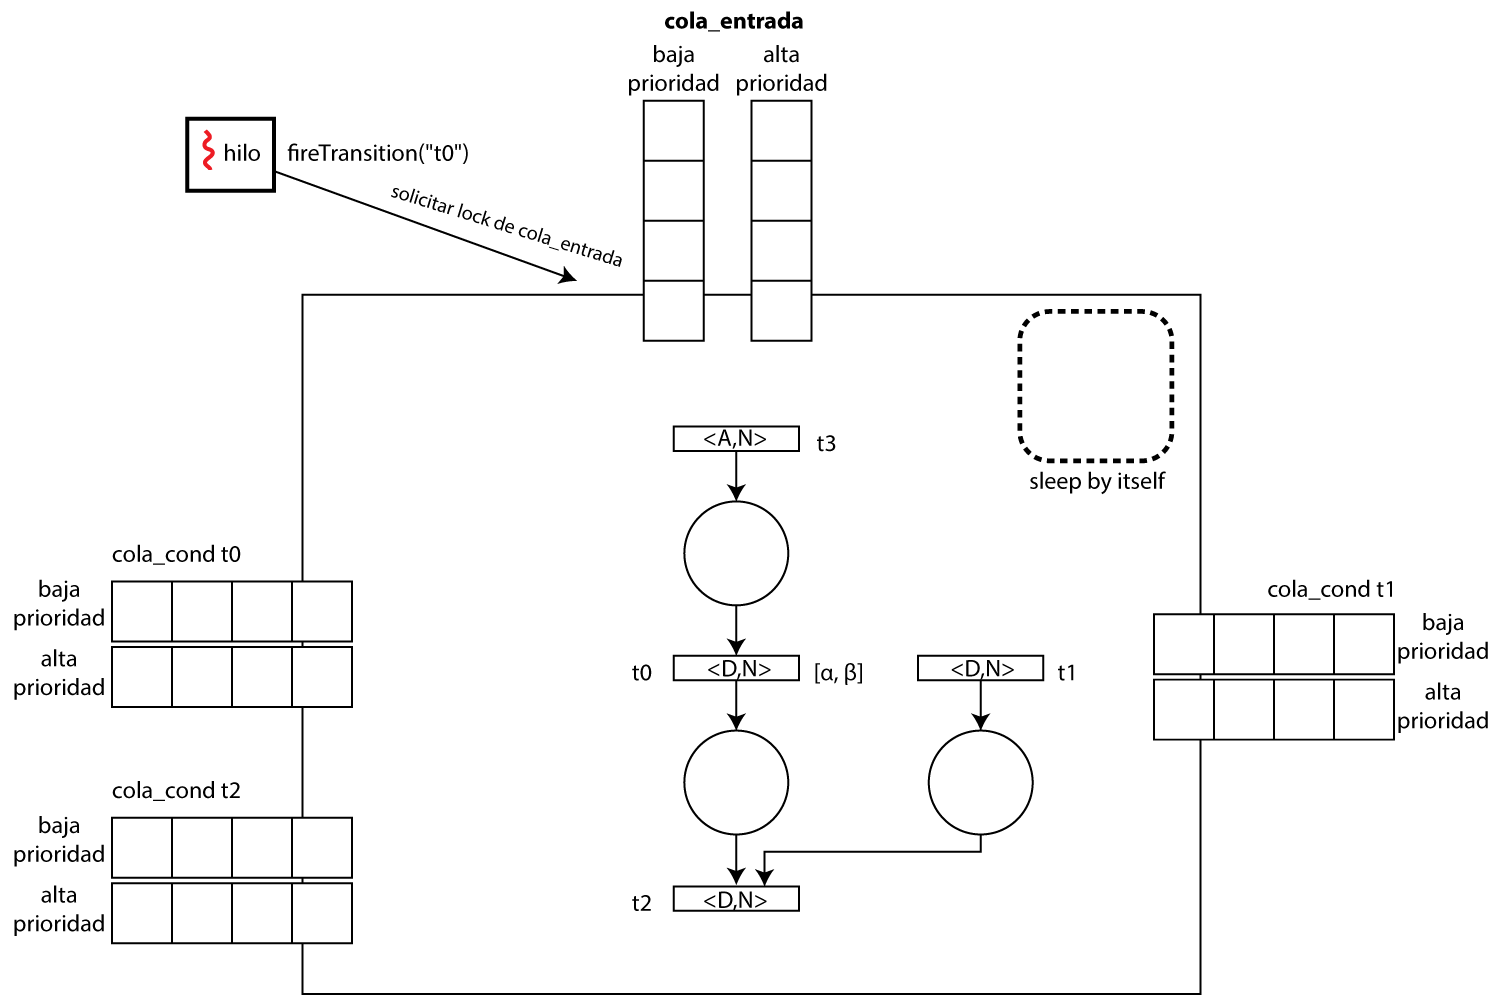
\includegraphics[width=\textwidth]{InversionPrioridad/solucion/Solucion_Inversion_Prioridad_01}
    }
    \label{fig:Inv_prior_entrada}
    \phantomcaption
\end{figure}
\begin{figure}[H]
    \centering
    \ContinuedFloat
    \subfigure[] {
      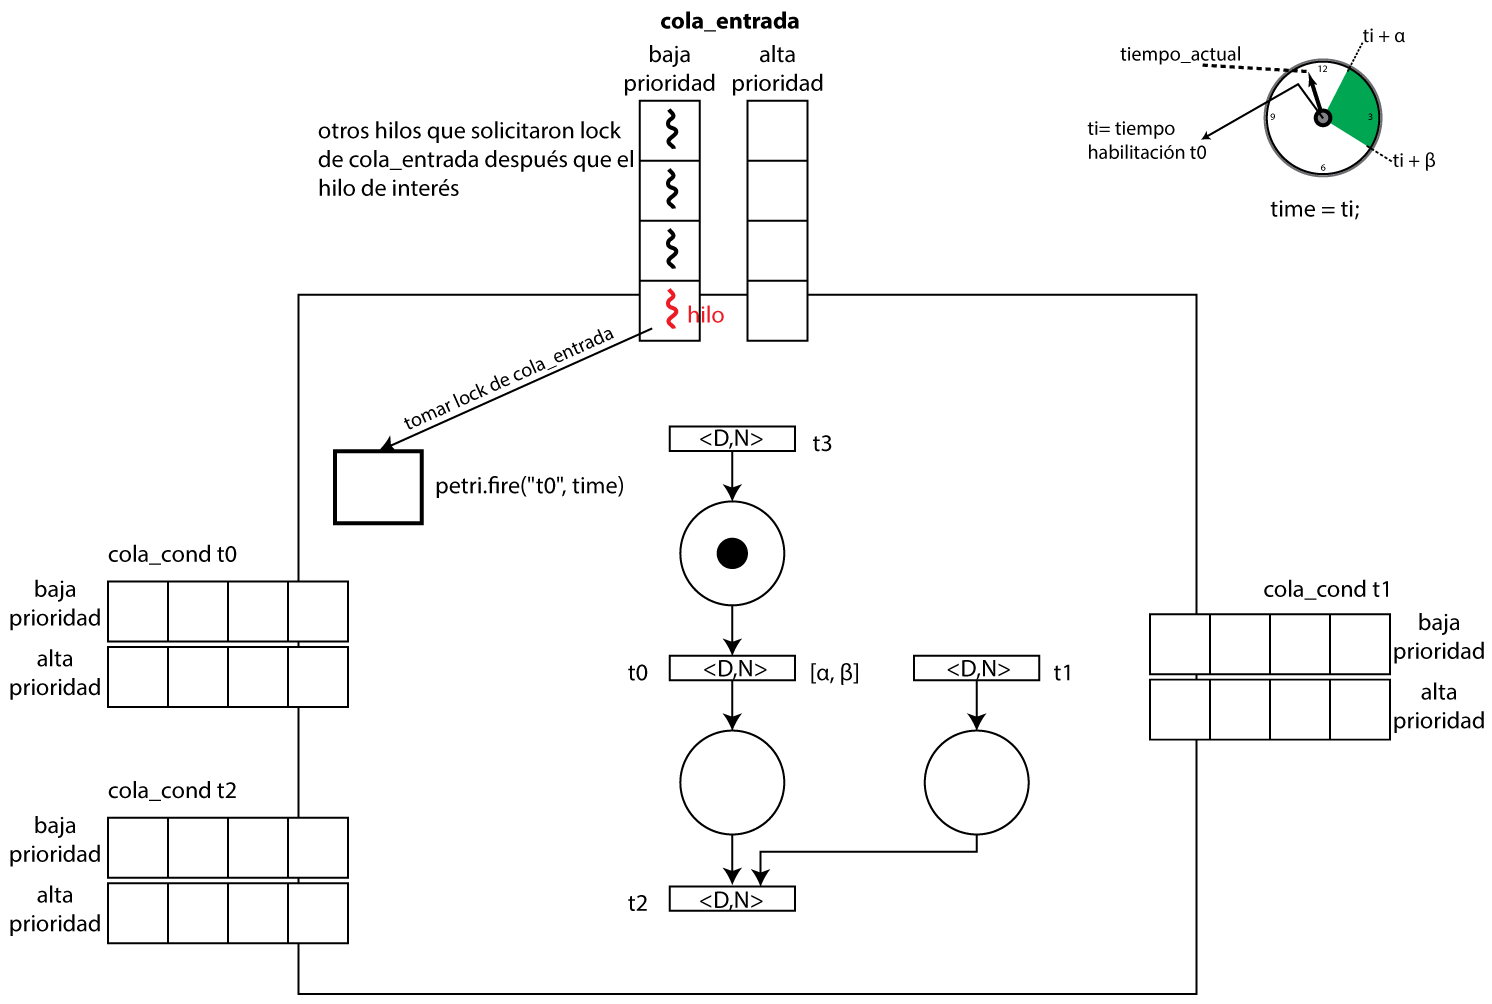
\includegraphics[width=\textwidth]{InversionPrioridad/solucion/Solucion_Inversion_Prioridad_02}
    }
    \label{fig:Inv_prior_entrada}
    \phantomcaption
\end{figure}
\begin{figure}[H]
    \centering
    \ContinuedFloat
    \subfigure[] {
      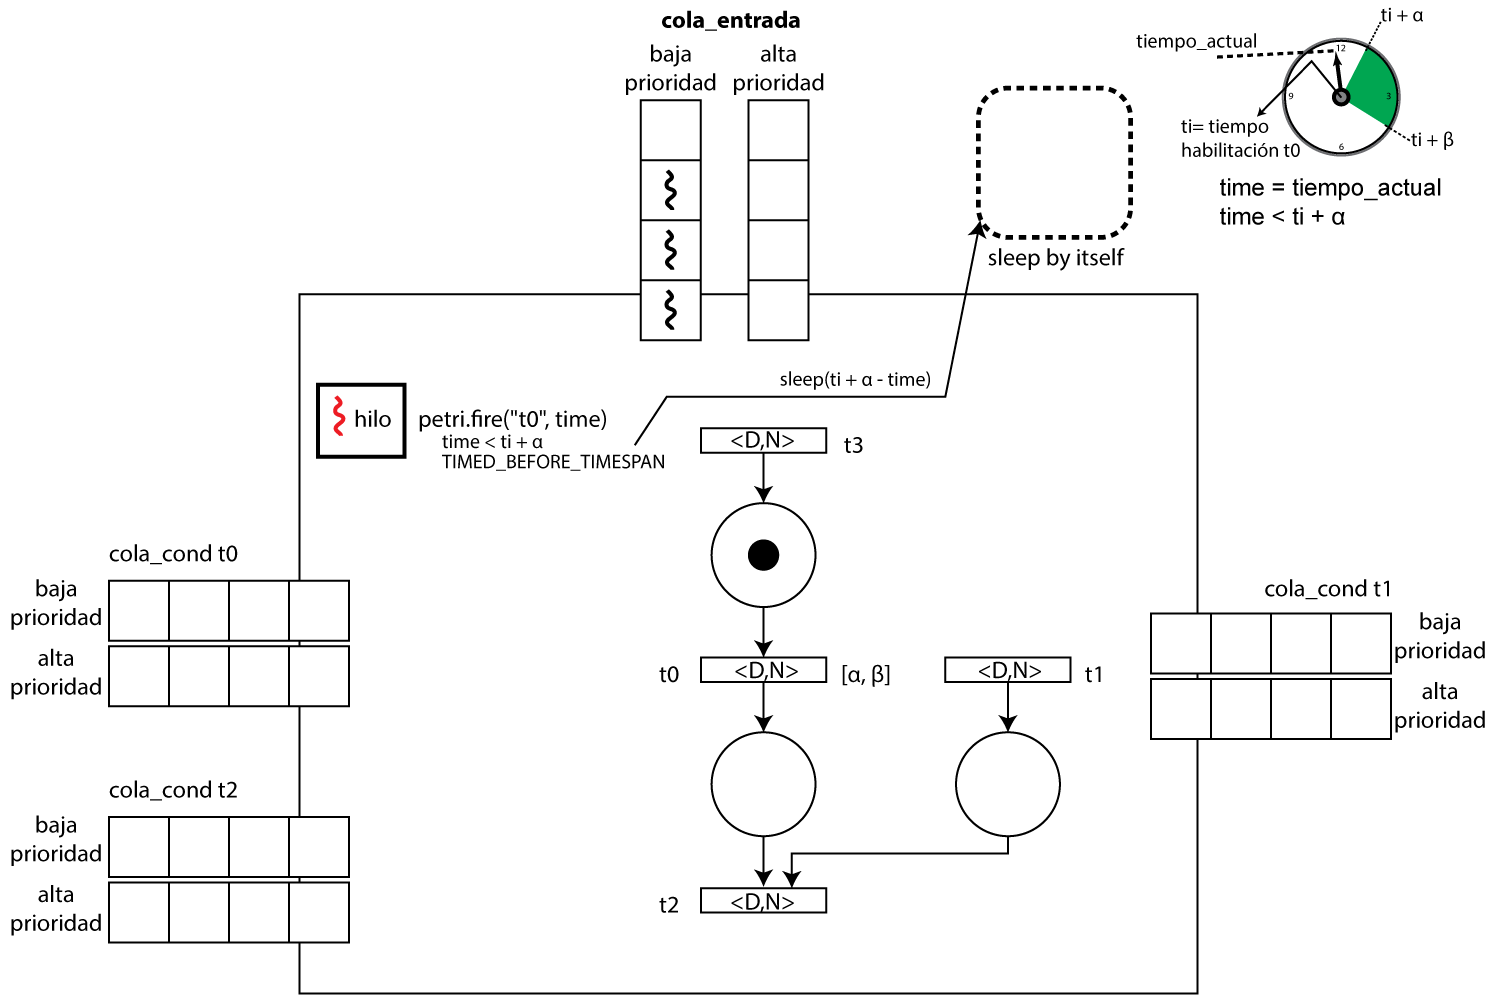
\includegraphics[width=\textwidth]{InversionPrioridad/solucion/Solucion_Inversion_Prioridad_03}
    }
    \label{fig:Inv_prior_entrada}
    \phantomcaption
\end{figure}
\begin{figure}[H]
    \centering
    \ContinuedFloat
    \subfigure[] {
      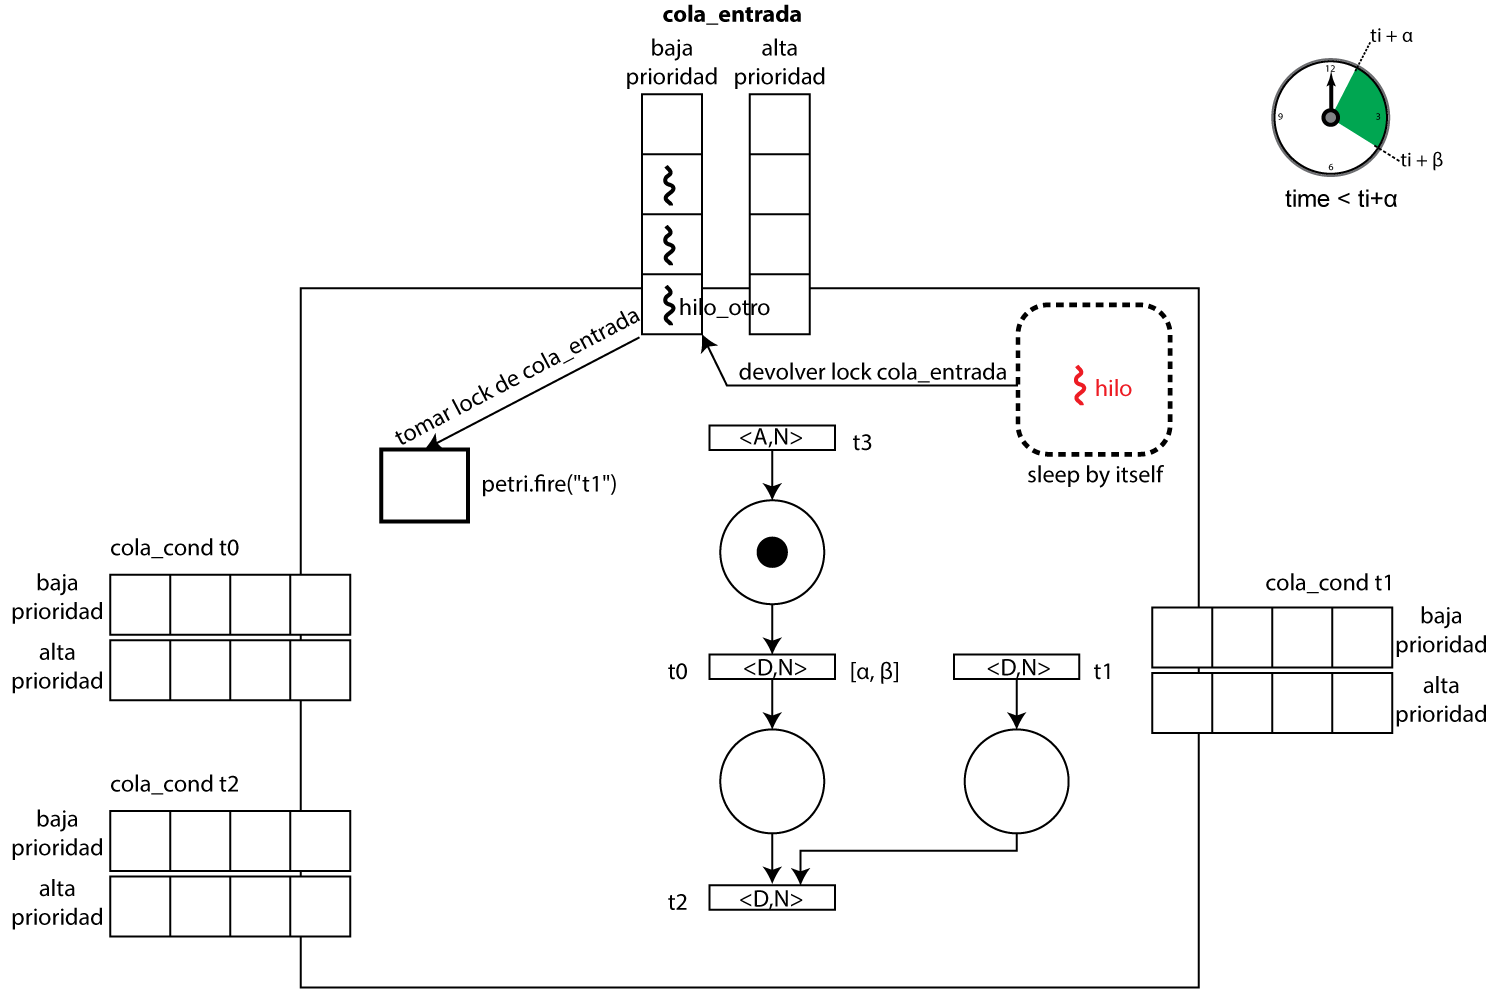
\includegraphics[width=\textwidth]{InversionPrioridad/solucion/Solucion_Inversion_Prioridad_04}
    }
    \label{fig:Inv_prior_entrada}
\end{figure}
\begin{figure}[H]
    \centering
    \ContinuedFloat
    \subfigure[] {
      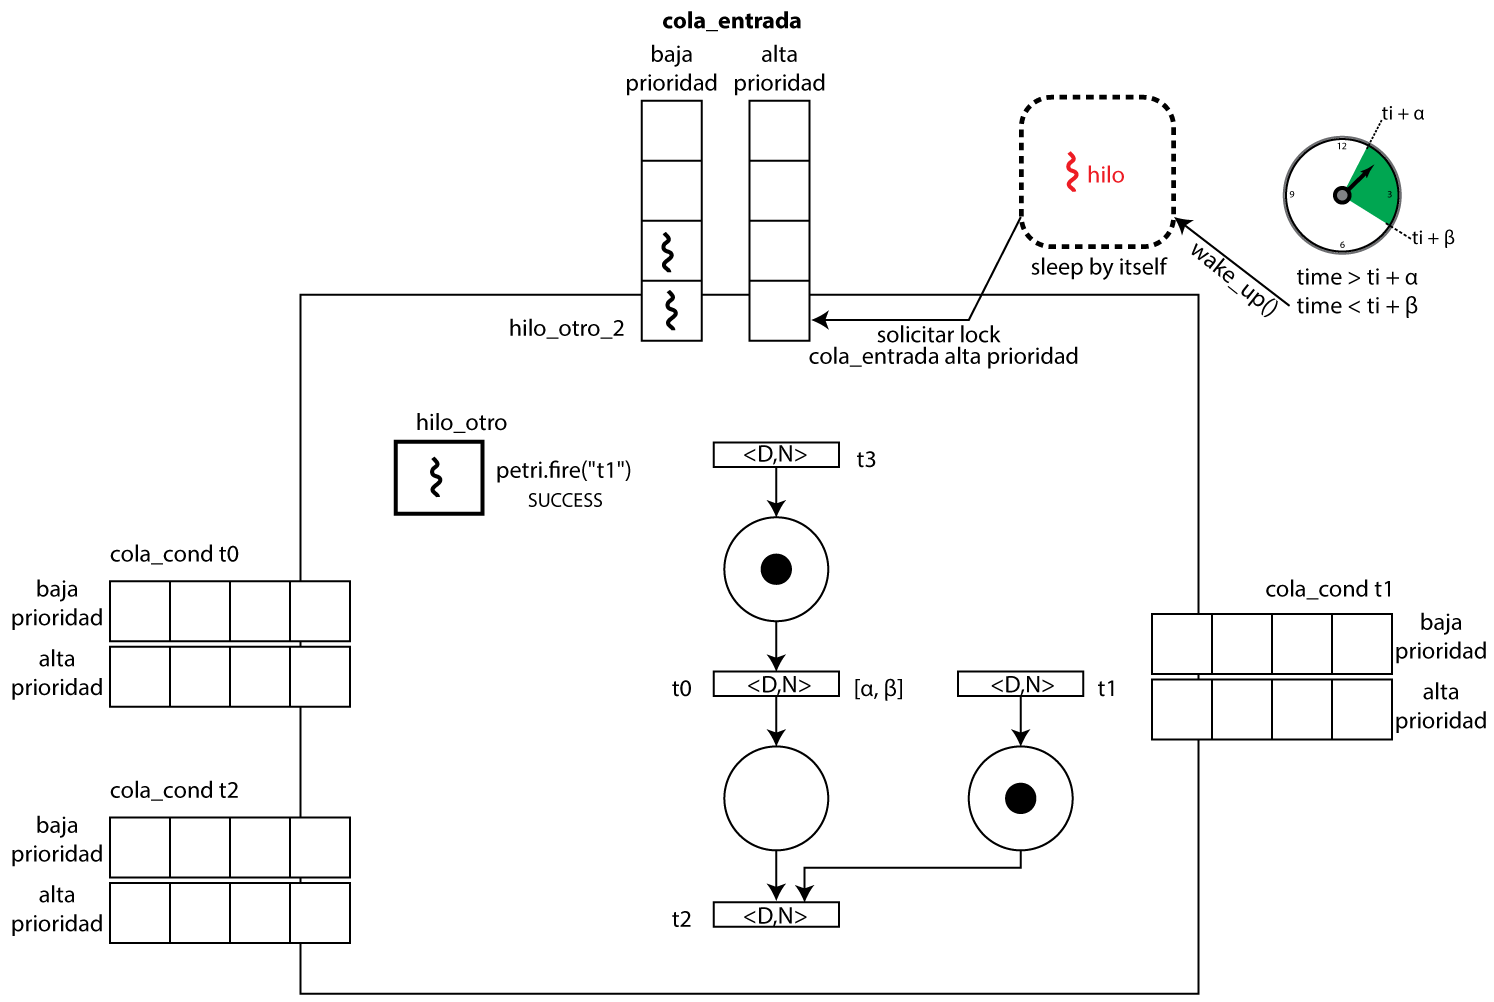
\includegraphics[width=\textwidth]{InversionPrioridad/solucion/Solucion_Inversion_Prioridad_05}
    }
    \label{fig:Inv_prior_entrada}
    \phantomcaption
\end{figure}
\begin{figure}[H]
    \centering
    \ContinuedFloat
    \subfigure[] {
      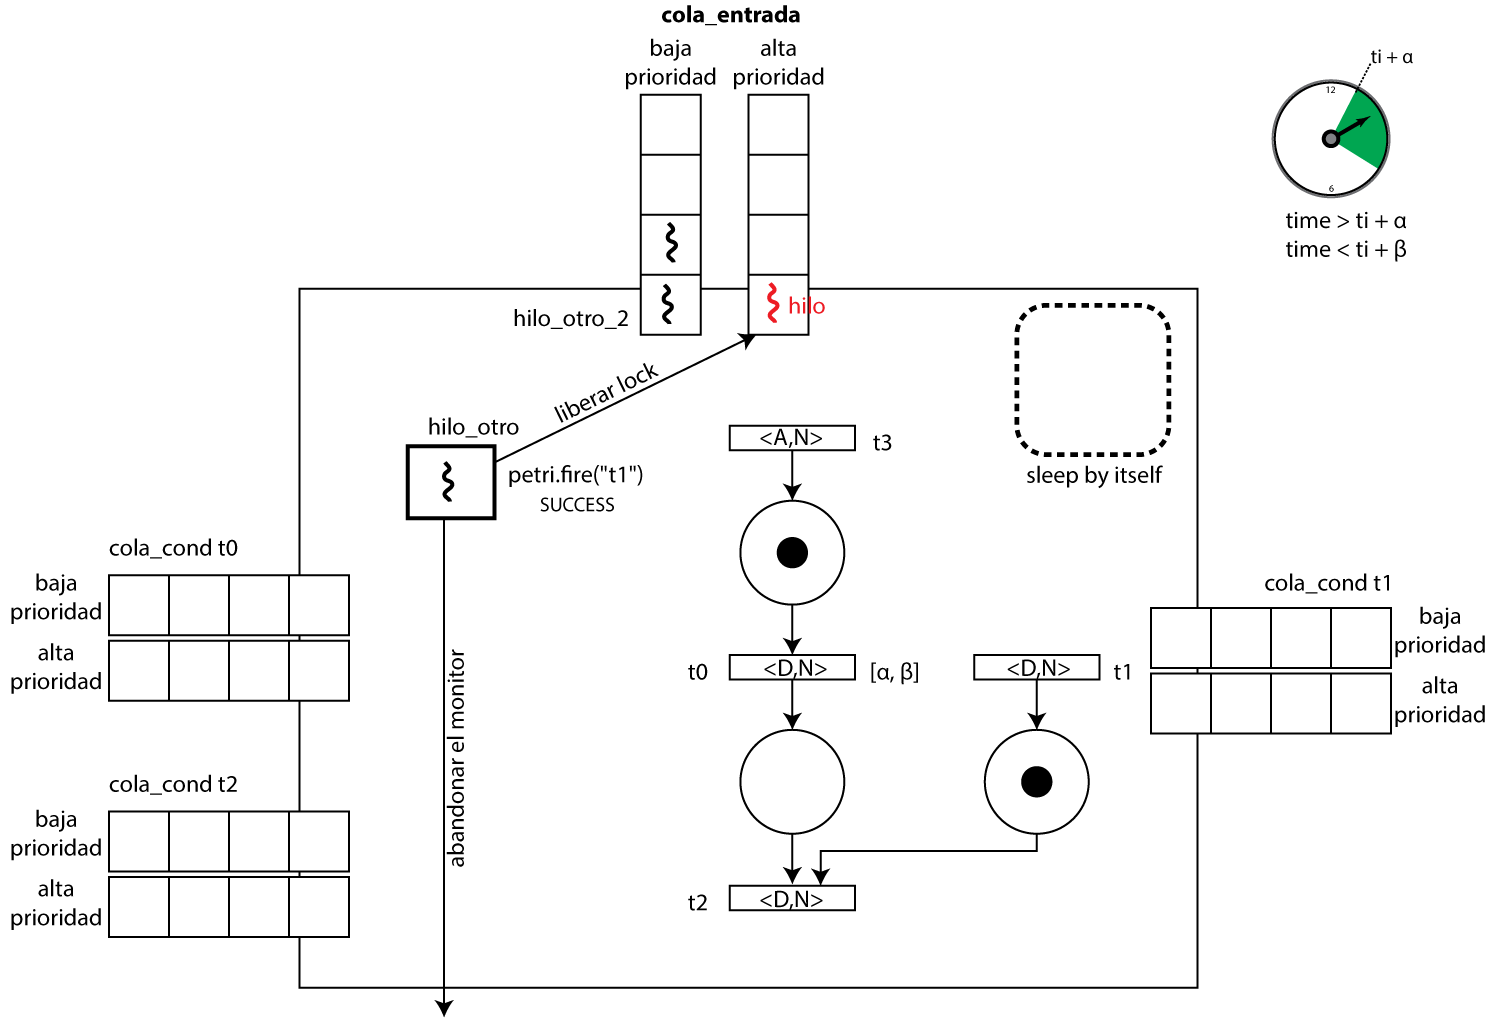
\includegraphics[width=\textwidth]{InversionPrioridad/solucion/Solucion_Inversion_Prioridad_06}
    }
    \label{fig:Inv_prior_entrada}
\end{figure}
\begin{figure}[H]
    \centering
    \ContinuedFloat
    \subfigure[] {
      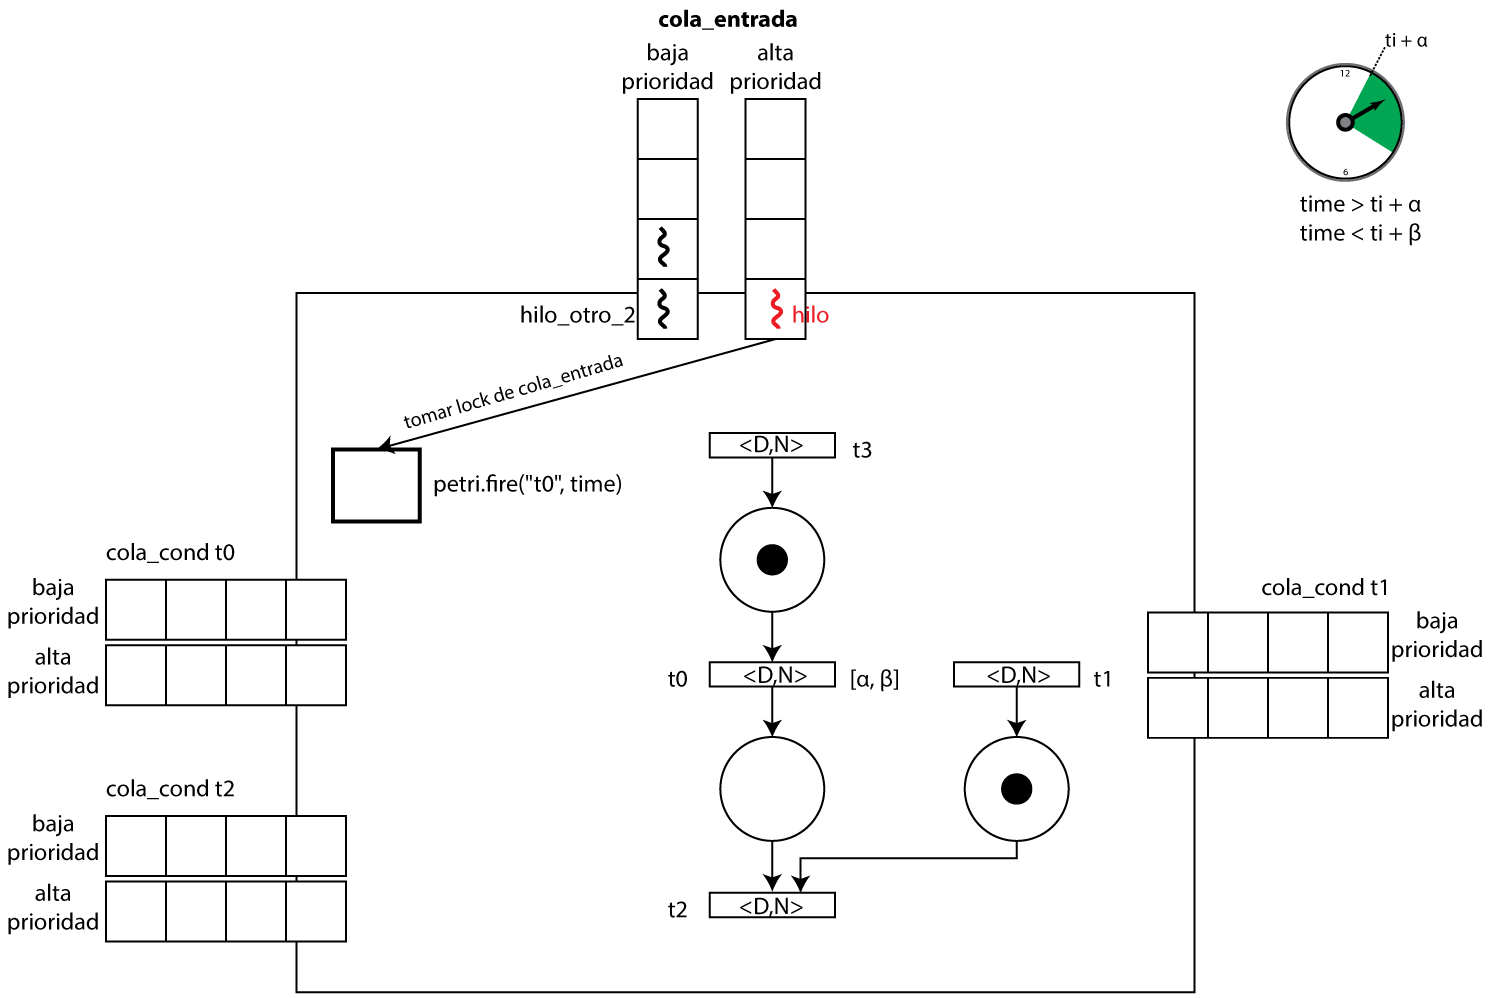
\includegraphics[width=\textwidth]{InversionPrioridad/solucion/Solucion_Inversion_Prioridad_07}
    }
    \label{fig:Inv_prior_entrada}
    \phantomcaption
\end{figure}
\begin{figure}[H]
    \centering
    \ContinuedFloat
    \subfigure[] {
      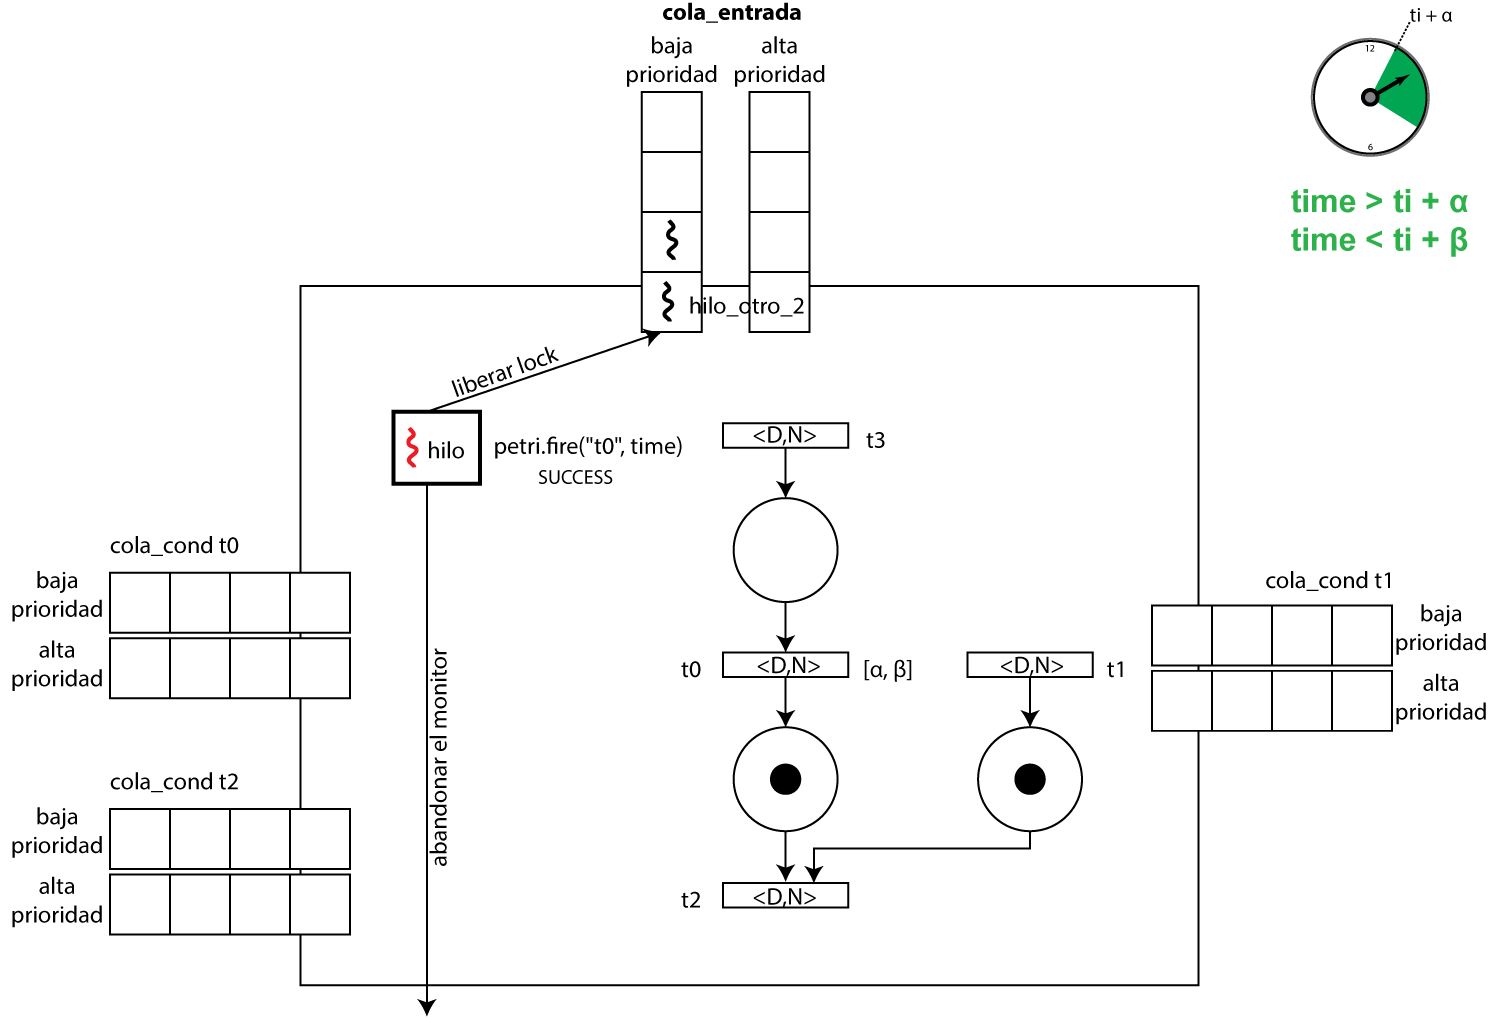
\includegraphics[width=\textwidth]{InversionPrioridad/solucion/Solucion_Inversion_Prioridad_08}
    }
    \caption{Inversión de prioridades en la cola de entrada del monitor}
    \label{fig:Inv_prior_entrada}
\end{figure}

\subsection{Informes de Disparo de una Transición}

Existen casos en los que es de interés del programador de un sistema que
utilice a JPCM recibir una notificación cuando se produce el disparo de una
transición. Para esto, JPCM ofrece una interfaz de suscripción a eventos de
disparo de transición.

Como se puede observar en el diagrama de la figura \ref{fig:JPCM_Fire_SUCCESS},
luego de un disparo exitoso se envía un evento de disparo. Para que un
observador reciba este evento debe haberse suscrito previamente a los eventos de
la transición en cuestión. La suscripción se realiza con una llamada al método
\mint{java}|PetriMonitor.subscribeToTransition()|.

Un intento de suscripción a una transición que no sea de tipo \textit{informada}
resulta en el lanzamiento de una excepción \mint{java}|IllegalArgumentException|
con un mensaje que explica la situación. De la misma manera, no se realizan
envíos de eventos para transiciones que no sean de tipo \textit{informada}.

\subsection{Guardas}

Como se explicó en la sección \ref{guardas}, a una transición se pueden asociar
valores booleanos que modifican su semántica de sensibilización. JPCM provee
soporte para guardas con habilitación por valor \mint{java}|true| o por valor
\mint{java}|false|.

Las guardas son cargadas en tiempo de inicialización durante la construcción
del objeto \mint{java}|PetriNet| y son inicializadas con valor
\mint{java}|false|.

En cualquier momento un hilo puede modificar el valor de una guarda accediendo
al método\\ \mint{java}|PetriMonitor.setGuard()| con el nombre de la guarda a
modificar y su nuevo valor. Esto es coordinado por el lock de entrada de forma
conjunta con el disparo de una transición para evitar problemas de acceso
concurrente sobre la RdP. Se contempla la posible sensibilización de
transiciones, ya sean de tipo \textit{automática} (donde el hilo que hizo el
cambio de valor de la guarda realiza el disparo) o de tipo \textit{disparada}
(en cuyo caso desbloquea a un hilo que estuviera esperando en su cola de
condición si lo hubiera) de la misma forma que en el disparo de una transición.
